% -*- TeX:UTF-8 -*-
%%
%% KAIST 학위논문양식 LaTeX용 (ver 0.5) 예시
%%
%% @version 0.4
%% @author  채승병 Chae,Seungbyung (mailto:chess@kaist.ac.kr)
%% @date    2004. 11. 12.
%%
%% @requirement
%% teTeX, fpTeX, teTeX 등의 LaTeX2e 배포판
%% + 은광희 님의 HLaTeX 0.991 이상 버젼 또는 홍석호 님의 HPACK 1.0
%% : 설치에 대한 자세한 정보는 http://www.ktug.or.kr을 참조바랍니다.
%%
%% @note
%% 기존에 널리 쓰여오던 차재춘 님의 학위논문양식 클래스 파일의 형식을
%% 따르지 않고 전면적으로 다시 작성하였습니다. 논문 정보 입력부분에서
%% 과거 양식과 다른 부분이 많으니 아래 예시에 맞춰 바꿔주십시오.
%%
%%
%% @acknowledgement
%% 본 예시 논문은 물리학과 박사과정 김용현 님의 호의로 제공되었습니다.
%%
%% -------------------------------------------------------------------
%% @information
%% 이 예제 파일은 hangul-ucs를 사용합니다. UTF-8 입력 인코딩으로
%% 작성되었습니다. hlatex의 hfont는 이용하지 않습니다. --2006/02/11
%% 본 템플릿은 전산학부 김민혁 교수에의해서 버그 수정되었습니다. -- 2016/11/25

% @class kaist.cls
% @options [default: doctor, korean, final]
% - doctor: 박사과정 | master : 석사과정
% - korean: 한글논문 | english: 영문논문
% - final : 최종판   | draft  : 시험판
% - pdfdoc : 선택하지 않으면 북마크와 colorlink를 만들지 않습니다.

\documentclass[master,english,final]{kaist-ucs}
\usepackage{float} 
\usepackage{subcaption}
\usepackage{graphicx}
\usepackage{amsfonts}
\usepackage{algorithm}
\usepackage{algorithmic}
\usepackage{multirow}
\usepackage{mathtools}
\usepackage{enumitem}

\usepackage{tabularx}

\usepackage{booktabs}      % \toprule, \midrule, \bottomrule 등 표 꾸미기
\usepackage{makecell}      % \makecell{} 사용 가능 (셀 내부 줄바꿈 등)
\usepackage{amsmath}       % 수식 정렬 등 수학 관련 기능
\newcommand{\ie}{\textit{i.e.}}
\newcommand{\eg}{\textit{e.g.}}
% If you want make pdf document (include bookmark, colorlink)
% \documentclass[doctor,english,final,pdfdoc]{kaist-ucs}

% kaist.cls 에서는 기본으로 dhucs, ifpdf, graphicx 패키지가 로드됩니다.
% 추가로 필요한 패키지가 있다면 주석을 풀고 적어넣으십시오,
%\usepackage{...}


% @command title 논문 제목(title of thesis)
% @options [default: (none)]
% - korean: 한글제목(korean title) | english: 영문제목(english title)
\title[korean] {조합적 추론을 통한 비전-언어 모델의 다중 이미지 암묵적 유해성 진단 및 완화}
\title[english]{Diagnosing and Mitigating Implicit Multi-Image Harm in Vision-Language Models through Compositional Reasoning}

% @note 표지에 출력되는 제목을 강제로 줄바꿈하려면 \linebreak 을 삽입.
%       \\ 나 \newline 등을 사용하면 안됩니다. (아래는 예시)
%
%\title[korean]{탄소 나노튜브의 물리적 특성에 대한\linebreak 이론 연구}
%\title[english]{Theoretical study on physical properties of\linebreak
%                carbon nanotubes}
%
% If you want to begin a new line in cover, use \linebreak .
% See examples above.
%


% @command author 저자 이름
% @param   family_name, given_name 성, 이름을 구분해서 입력
% @options [default: (none)]
% - korean: 한글이름 | chinese: 한문이름 | english: 영문이름
% 한문 이름이 없다면 빈 칸으로 두셔도 됩니다.
%
%
% If you are a foreigner , write your name in korean or your korean name.
% If you can't write native character, you can make the chinese blank empty 
% Write as follow
% \author[korean]{family name in korean}{given name in korean}
% \author[chinese]{family name in your native language}{given name in your native language}
% \author[english]{family name in english}{given name in english}
%
\author[korean]{정}{욱 연}
\author[korean2]{정}{욱연}    %이름을 붙여 써 주시기 바랍니다.
\author[chinese]{鄭}{旭 然}
\author[english]{Zheng}{Xuran}

% @command advisor 지도교수 이름 (복수가능)
% @usage   \advisor[options]{...한글이름...}{...영문이름...}{signed|nosign}
% @options [default: major]
% - major: 주 지도교수  | coopr: 공동 지도교수
\advisor[major]{유 창 동}{Chang D. Yoo}{signed}
\advisor[major2]{유창동}{Chang D. Yoo}{signed}    %한글 성과 한글 이름을 모두 붙여 써 주시기 바랍니다.
\advisorinfo{Professor of Electrical Engineering} %제출승인서에 들어가는 교수님 정보, advisor's information 
%\advisor[coopr]{홍 길 동}{Gil-Dong Hong}{nosign}
%\advisor[coopr2]{홍길동}{Gil-Dong Hong}{nosign}    %한글 성과 한글 이름을 모두 붙여 써 주시기 바랍니다.
%
% 지도교수 한글이름은 입력하지 않아도 됩니다.
% You may not input advisor's korean name
% like this \advisor[major]{}{Chang, Kee Joo}{signed}
%


% @command department {학과이름}{학위종류} - 아래 규칙에 따라 코드를 입력
% @command department {department code}{degree field}
%
% department code
% 2. 석박사학위논문 작성 및 제출요령 4쪽 ~ 5쪽 참고
% 또는 kaist-ucs.cls 의 % @command department 참고

% science: 이학 | engineering: 공학 | business : 경영학
% 박사논문의 경우는 학위종류를 입력하지 않아도 됩니다.
% If you write Ph.D. dissertation, you cannot input degree field.
% The third parameter : a | b | c
% a: 소속된 학과만 쓰는 옵션 (학과에만 소속되어 있는 경우에는 무조건 a를 선택해야 함)
% b: 학과 아래의, 프로그램이나 학제전공에 소속되어 있을 경우에 학과와 프로그램을 함께 쓰는 옵션
% c: 학과 아래의, 프로그램이나 학제전공에 소속되어 있을 경우에 학과를 쓰지 않고 프로그램이나 학제전공의 이름만 쓰는 옵션 
% 
% a: it represents only the name of department. (if you aren't in the program under the department, must choose a)
% b: it represents the names of department and the program that is under the department (consider this when you are in the program not only department)
% c: it represents only the name of program that is under the department (consider this when you are in the program not only department)
\department{EE}{engineering}{c}

% @command referee 심사위원 (석사과정 3인, 박사과정 5인)
\referee[1]{유 창 동}
\referee[2]{김 준 모}
\referee[3]{한 인 수}
%\referee[4]{가 동 호}
%\referee[5]{박 태 현}
% \referee[5] {Barack Obama}
% Of course english name is available

% @command approvaldate 지도교수논문승인일
% @param   year,month,day 연,월,일 순으로 입력
\approvaldate{2027}{12}{9}

% @command refereedate 심사위원논문심사일
% @param   year,month,day 연,월,일 순으로 입력
\refereedate{2027}{12}{9}

% @command gradyear 졸업년도
\gradyear{2027}

% 본문 시작
\begin{document}

    % 앞표지, 속표지, 학위논문 제출승인서, 학위논문 심사완료 검인서는
    % 클래스 옵션을 final로 지정해주면 자동으로 생성되며,
    % 반대로 옵션을 draft로 지정해주면 생성되지 않습니다.

    % 논문 서지, 초록, 핵심 낱말, 영문 초록, 영어 핵심 낱말 (Information of thesis, abstract in korean, keywords in korean, abstract in english, keywords in english)
   \thesisinfo
   %% Letters of abstract in korean must be less than 500 and words of abstract in english must be less than 300.
   %% Number of keywords must be less than 6.
   %% Don't write english letters in the abstract in korean.
    \begin{summary}           
    오프라인 강화학습은 환경과의 실시간 상호작용이 비용이 크거나 위험한 상황에서 고정된 데이터셋만으로 학습할 수 있다는 점에서 매력적인 대안이다. 그러나 오프라인 데이터셋을 위한 보상 함수 설계에는 상당한 인력과 도메인 전문성이 요구된다. 인간 피드백 기반 강화학습(RLHF)은 수작업 보상 설계의 대안으로 부상했지만, 지속적인 인간 개입이 필요해 비용 부담이 크며 자동화된 보상 생성에 대한 수요를 키우고 있다. 우리는 인간 개입 없이 오프라인 데이터로부터 보상을 자동 생성하기 위해 대형 비전-언어 모델의 추론 능력을 활용하는 RG-VLM을 제안한다. RG-VLM은 조밀한 보상 생성을 통해 장기 과제에서의 일반화를 개선하고, 희소 보상과 결합될 때 보조 보상 신호로서 추가적인 성능 향상을 제공한다. 또한 간단한 프롬프트 기반 절차로 다양한 데이터셋 전반에 확장가능하다. 실험적으로는 희소 보상만 사용하는 기준선 대비 일관된 성능 향상과 수작업 보상 설계 의존도의 감소를 확인했으며, 기존 비전-언어모델 기반 보상 생성 기법보다도 더 높은 성능을 기록했다. RG-VLM은 오프라인 강화학습에서 저비용, 확장 가능한 보상 생성을 제공한다. 
    \end{summary}
   
    \begin{Korkeyword}
    오프라인 강화학습, 대형 비전-언어 모델 , 보상 라벨링
    \end{Korkeyword}


    \begin{abstract}
    Offline reinforcement learning offers a compelling alternative in settings where real-time interaction is costly or risky by learning solely from fixed datasets. However, designing reward functions for offline datasets demands substantial human effort and domain expertise. Reinforcement learning with human feedback (RLHF) has emerged as an alternative to handcrafted shaping, but its reliance on human involvement is costly, increasing the demand for automated reward generation. We propose RG-VLM, which leverages the reasoning capabilities of large vision–language models to automatically generate rewards from offline data without human intervention. By generating dense reward signals, RG-VLM improves generalization on long-horizon tasks and, when combined with sparse rewards, serves as an auxiliary signal that further boosts performance. Moreover, a simple prompt-based procedure makes the approach scalable across diverse datasets. Empirically, RG-VLM delivers consistent improvements over sparse-only baselines and reduces reliance on handcrafted reward design, while outperforming prior vision-language model based reward generation methods. RG-VLM thus provides low-cost, scalable reward generation for offline reinforcement learning.

    \end{abstract} 
     
    \begin{Engkeyword}
    Offline Reinforcement Learning, Large Vision-Language Model, Reward labeling
    \end{Engkeyword}
   

    \addtocounter{pagemarker}{1}                 % 백색별지분을 고려
    \newpage 
  


    % 목차 (Table of Contents) 생성
    \tableofcontents

    % 표목차 (List of Tables) 생성
    \listoftables

    % 그림목차 (List of Figures) 생성
    \listoffigures

    % 위의 세 종류의 목차는 한꺼번에 다음 명령으로 생성할 수도 있습니다.
    %\makecontents

%% 이하의 본문은 LaTeX 표준 클래스 report 양식에 준하여 작성하시면 됩니다.
%% 하지만 part는 사용하지 못하도록 제거하였으므로, chapter가 문서 내의
%% 최상위 분류 단위가 됩니다.
%% You cannot use 'part'

\chapter{Introduction}
\noindent

\begin{figure}[H]
    \centerline{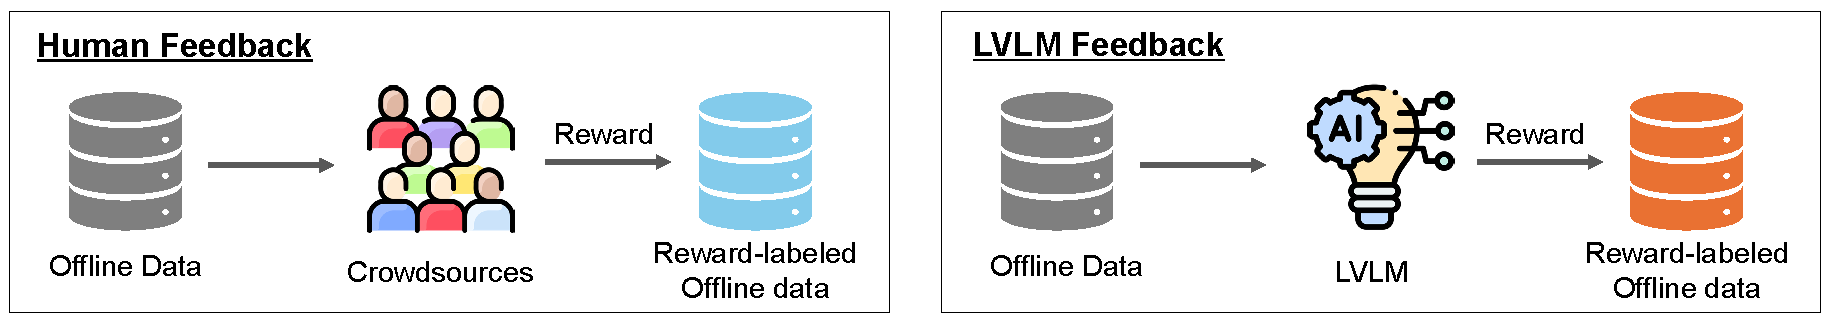
\includegraphics[width=16cm]{figures/figure1.pdf}}
    \caption[Comparison between Human Feedback and LVLM Feedback in reward labeling.]{Comparison between Human Feedback and LVLM Feedback in reward labeling. Unlike human feedback-based methods, LVLM feedback leverages the advanced reasoning capabilities of large vision-language models (LVLMs) to automatically generate rewards, removing the need for human involvement} \label{fig:compare_method}
\end{figure}

Goal-conditioned offline reinforcement learning (RL) has emerged as a promising approach for applying deep RL in domains where real-time interaction with the environment is costly or impractical \cite{prudencio2023survey}, such as robotics \cite{singh2022reinforcement}, healthcare \cite{liu2020reinforcement}, and autonomous driving \cite{kiran2021deep}. Unlike online RL, where agents continuously interact with the environment, offline RL operates on fixed datasets, making it an attractive solution for scenarios where data collection is expensive or risky. To prevent distribution shifts between the offline dataset and the learned policy \cite{levine2020offline}, offline RL methods typically incorporate conservative learning objectives alongside value-based methods \cite{fujimoto2019off,kumar2020conservative,liu2020provably}. One of the central challenges in goal-conditioned offline RL is the sparsity of the reward signal \cite{andrychowicz2017hindsight,luu2021hindsight,ma2022offline,luu2024predictive}, where agents are unable to explore the environment to uncover informative states that align with the desired goals. Moreover, shaping a reward function to extract reward signals from the offline dataset may require extensive human effort and deep domain expertise \cite{zhu2023scaling,hadfield2017inverse}, and these handcrafted reward functions may still fail to fully reflect human intentions. 

Recently, reinforcement learning with human feedback (RLHF) has garnered increasing attention as a powerful paradigm that transforms human feedback into guidance signals, eliminating the need to manually design reward functions \cite{lee2021pebble, yuan2024uni, hiranaka2023primitive}. However, RLHF often requires a human-in-the-loop during the training of RL agents, which is costly. To address this, previous works have focused on learning a reward model to capture human preferences based on selected trajectories \cite{lee2021pebble, peng2020learning, xue2023reinforcement}. While promising, these methods still require human labeling on an initial dataset, which may lack flexibility when transferring to new tasks. Meanwhile, Large Vision-Language Models (LVLMs) trained on massive, Internet-scale datasets have demonstrated exceptional capabilities in solving complex reasoning problems \cite{alayrac2022flamingo,liu2024improved,reid2024gemini,achiam2023gpt}. Recent works have attempted to leverage LVLMs to tackle different aspects of the RL problem, such as generating planners \cite{ahn2022can,huang2022language}, discovering skills \cite{du2023guiding,zhang2023bootstrap}, or fine-tuning LVLMs for direct use as policies \cite{szot2023large,zhai2024fine}. 

Motivated by these successes, and to address the challenge of approximating ground truth rewards in offline data, we propose \textbf{R}eward \textbf{G}eneration via L\textbf{VLM} (RG-VLM), a novel approach that leverages a pre-trained LVLM to generate rewards for previously collected data. In contrast to RLHF-based methods, RG-VLM eliminates the need for human involvement during the reward labeling process, as illustrated in Fig. \ref{fig:compare_method}, thereby offering a more scalable and flexible approach for generating rewards in new tasks. By harnessing the advanced reasoning capabilities of LVLM, RG-VLM generates interpretable dense rewards, providing more informative feedback and leading to improved performance in complex tasks.  To summarize, the key contributions of our work are:
\begin{enumerate}
    \item We introduce RG-VLM, a novel approach that leverages Large Vision-Language Models (LVLMs) to generate rewards from offline data, eliminating the need for human labeling and manual reward design.
    \item We demonstrate that RG-VLM enhances policy generalization across diverse long-horizon tasks, showing robust in varying environments and task complexities. 
    \item Our ablation study shows that combining RG-VLM with sparse rewards improves performance compared to using RG-VLM alone, highlighting its potential as an auxiliary reward signal to enhance traditional sparse rewards. 
\end{enumerate}

%%%%%%%%%%%%%%%%%%%%%%%%%%%%%%%%%%%%%%%%%%%%%%%%%%%%

\chapter{Preliminary}

\section{Offline Reinforcement Learning}

\begin{figure}[H]
    \centerline{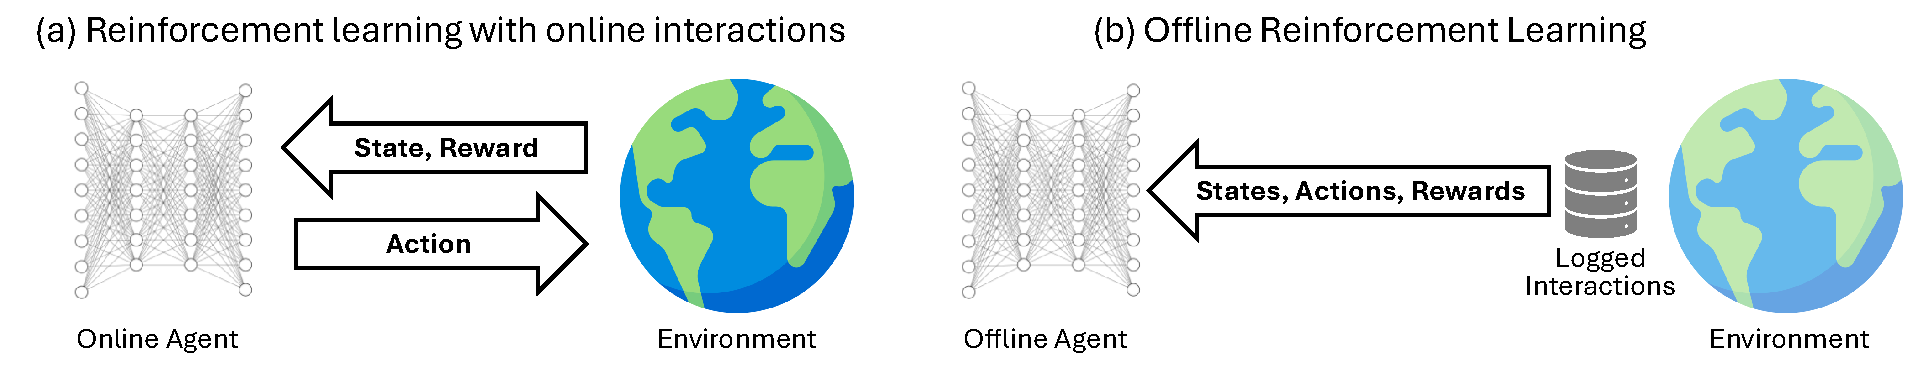
\includegraphics[width=16cm]{figures/figure2.pdf}}
      \caption{
  Comparison of reinforcement learning with online interactions and offline reinforcement learning. (a) In online reinforcement learning, the agent repeatedly acts in the environment and receives states and rewards to update its policy. (b) In offline reinforcement learning, the agent learns from a fixed dataset of logged interactions that includes states, actions, and rewards with no additional environment access during training.}
  \label{fig:offline_rl}
\end{figure}

% Offline reinforcement learning (RL) studies how to learn policies solely from a fixed dataset of prior interactions, with no further environment access during training, as illustrated in Figure \ref{fig:offline_rl}. Formally, an offline dataset $D=\{(s,a,r,s')\}$ is collected by a behavior policy $\pi_\beta$, and the learner seeks a policy $\pi_{off}$ that maximizes expected return while never querying the environment. This setting is attractive when online interaction is costly, risky, or impractical (e.g., robotics\cite{singh2022reinforcement}, healthcare\cite{liu2020reinforcement}, or autonomous driving\cite{kiran2021deep}) and is distinct from both online and off-policy RL which still gather new data.

% Learning from a static dataset is the key benefit of offline RL, yet it is also the reason why many online off-policy algorithms struggle in this setting. In theory, any off-policy method could be trained on previously collected experiences. However, in practice these methods often fail when used strictly offline since they were designed with the assumption that further environment interaction can correct erroneous behavior. The core challenge is to balance broader generalization with the need to avoid actions that fall outside the dataset distribution. High-capacity function approximators intensify this problem. Much of the recent offline RL literature tackles this issue by introducing losses and procedures that explicitly mitigate distribution shift.

% One direct approach constrains the learned policy toward the behavior policy that generated the data\cite{fujimoto2019off, kumar2019stabilizing, wu2019behavior}. Another line of work reduces risk by learning conservative value functions that underestimate returns on out-of-distribution state–action pairs, which discourages optimistic extrapolation\cite{kumar2020conservative, yu2021combo}. Model-based methods often estimate uncertainty with ensembles and penalize actions that produce inconsistent predictions, which promotes decisions that remain consistent across models \cite{janner2019trust, kidambi2020morel}. There are also strategies that do not impose an explicit constraint yet still curb distribution shift\cite{chen2020bail}. Examples include adding a behavior-cloning term to the policy update or adopting one-step objectives that limit iterative drift\cite{brandfonbrener2021offline, kostrikov2021offline}.

% By contrast, some approaches do not address distribution shift at all. Importance sampling\cite{zhang2020gendice, nachum2019algaedice, nachum2019dualdice} and trajectory optimization\cite{chen2021decision, janner2021offline} seek an optimal policy or an optimal trajectory distribution, but they do not include mechanisms to keep the learned policy within the support of the dataset. These methods can be effective under strong assumptions, yet they provide little protection when the learned policy proposes out-of-distribution actions.

% Finally, evaluation without interaction is itself a core challenge. Reliable off-policy evaluation (e.g., fitted-Q evaluation, importance-sampling variants, or model-based estimators) is required to select hyper-parameters and decide when to stop training, yet remains an open problem across diverse datasets and task properties.

Offline reinforcement learning (RL) studies how to learn policies solely from a fixed dataset of prior interactions, with no further environment access during training, as illustrated in Figure \ref{fig:offline_rl}. Formally, an offline dataset $D=\{(s,a,r,s')\}$ is collected by a behavior policy $\pi_\beta$, where $s$ denotes the state, $a$ the action, $r$ the scalar reward, and $s'$ the next state. and the learner seeks a policy $\pi_{\text{off}}$ that maximizes expected return while never querying the environment. This setting is attractive when online interaction is costly, risky, or impractical (e.g., robotics \cite{singh2022reinforcement}, healthcare \cite{liu2020reinforcement}, or autonomous driving \cite{kiran2021deep}) and is distinct from both online and off-policy RL which still gather new data.

Learning from a static dataset is the key benefit of offline RL, yet it is also the main reason why many standard off-policy algorithms struggle in this setting. In online RL, the agent can correct erroneous value estimates or poor policies by collecting new experience in regions where its predictions are inaccurate. In offline RL, however, the policy must be learned entirely from fixed data, so any extrapolation beyond the state–action distribution covered by $D$ can lead to severe overestimation of Q-values and catastrophic exploitation. This distribution shift between the behavior policy $\pi_\beta$ and the learned policy $\pi_{\text{off}}$ is therefore the central challenge in offline RL \cite{levine2020offline}.

Most offline RL algorithms can be broadly categorized into model-based and model-free approaches, depending on whether they explicitly learn a dynamics model. Model-based offline RL methods first fit a transition model $\hat{p}(s' \mid s,a)$ from the dataset, and then optimize a policy inside this learned model. Since the model is only reliable in regions well supported by the data, these methods incorporate pessimism or uncertainty penalties to avoid exploiting model errors. For example, MOReL\cite{kidambi2020morel} constructs a pessimistic MDP by treating uncertain regions as absorbing failure states with large negative reward, thereby encouraging the policy to remain within the high-confidence region of the model. MOPO\cite{yu2020mopo} instead estimates model uncertainty using an ensemble and subtracts an uncertainty-dependent penalty from the reward, so that transitions with high epistemic uncertainty become less attractive to the policy. COMBO\cite{yu2021combo} further combines model-generated rollouts with real data while learning a conservative value function that lowers Q-values for out-of-distribution state–action pairs, effectively blending model-based exploration with value conservatism. These model-based approaches can leverage the dynamics model to generate additional synthetic experience, but must carefully control model bias to remain stable in the purely offline regime.

In contrast, model-free offline RL methods do not learn an explicit dynamics model. Instead, they directly learn value functions and policies from the dataset while modifying the learning objective to mitigate distribution shift. A prominent line of work is conservative value learning, where the algorithm explicitly penalizes large Q-values on actions that are unlikely under the behavior distribution. Conservative Q-Learning (CQL)\cite{kumar2020conservative} adds a regularization term that pushes up the Q-values for actions in the dataset while pushing down Q-values for actions outside the dataset support, ensuring that the learned value function is pessimistic in under-sampled regions. Another approach, BEAR (Bootstrapping Error Accumulation Reduction)\cite{kumar2019stabilizing}, constrains the learned policy to remain close to the behavior policy by penalizing distributional divergence between the policy’s action distribution and the actions observed in the dataset, thereby limiting extrapolation to unseen actions. More recently, Implicit Q-Learning (IQL)\cite{kostrikov2021offline} avoids querying out-of-distribution actions altogether by learning a value function via expectile regression and extracting the policy through advantage-weighted regression over actions observed in the dataset. These model-free methods are often simpler to implement than model-based ones and avoid compounding model errors, while still directly addressing the distribution shift problem at the level of value and policy learning.

Beyond these mainstream approaches, other lines of work explore importance-sampling-based objectives and sequence-modeling or trajectory-optimization formulations that treat policy learning as learning an optimal trajectory distribution \cite{zhang2020gendice, nachum2019dualdice, chen2021decision, janner2021offline}. However, these methods typically provide weaker safeguards against out-of-distribution actions unless strong assumptions on coverage or function approximation hold. Moreover, reliable evaluation without further interaction remains an open challenge: off-policy evaluation methods such as fitted Q-evaluation, importance-sampling variants, and model-based estimators are crucial for model selection and hyper-parameter tuning in offline RL, yet their accuracy can vary significantly across datasets and task properties \cite{levine2020offline}.

In the following subsections, we discuss representative model-based methods (MOReL\cite{kidambi2020morel}, MOPO\cite{yu2020mopo}, COMBO\cite{yu2021combo}) and model-free methods (CQL\cite{kumar2020conservative}, BEAR\cite{kumar2019stabilizing}, IQL\cite{kostrikov2021offline}) in more detail, highlighting how each addresses the distribution shift problem and how they relate to our use of IQL\cite{kostrikov2021offline} as the underlying offline RL algorithm in this work.

\subsection{Model-based Offline Reinforcement Learning}
Model-based offline RL methods first learn an explicit dynamics model from the offline dataset and then optimize a policy inside this learned model. Concretely, given a fixed dataset 
$D=\{(s,a,r,s')\}$ collected by a behavior policy $\pi_\beta$, where $(s,a,r,s')$ represent state, action, reward, and next-state tuples, these methods fit a parametric transition model $\hat{p}(s' |s,a)$ optionally together with a reward model $\hat{r}(s,a)$. Once the model has been trained, the agent can simulate rollouts using $\hat{p}$ instead of interacting with the real environment and perform planning or model-based policy optimization. This approach is attractive in the offline setting because it appears to circumvent the lack of environment access by generating synthetic experience. However, since $\hat{p}$ is only reliable in regions of the state–action space that are sufficiently covered by the dataset, model-based offline RL must explicitly address model bias. Inaccurate predictions in poorly covered or out-of-distribution regions can compound over multiple model rollouts and lead to severe overestimation of returns if not handled carefully. As a result, recent model-based offline RL algorithms are typically built around the idea of combining model learning with some notion of pessimism or uncertainty awareness in order to avoid exploiting model errors.

A representative example of this line of work is MOReL\cite{kidambi2020morel}, which constructs a pessimistic Markov decision process (MDP) based on a learned dynamics ensemble. MOReL\cite{kidambi2020morel} trains an ensemble of transition models on the dataset and uses the disagreement among ensemble members as a proxy for epistemic uncertainty. States and actions that lie in well-covered regions of the dataset exhibit low ensemble variance, whereas those that are rarely or never observed yield high disagreement. MOReL\cite{kidambi2020morel} then builds an augmented MDP in which highly uncertain transitions are redirected to an absorbing “failure” state with a large negative reward. Intuitively, this pessimistic MDP encodes the assumption that actions venturing into unknown regions are likely to lead to catastrophic outcomes. Standard planning or value iteration is then performed on this pessimistic MDP. Because the optimal policy in this modified MDP is discouraged from entering high-uncertainty regions, the resulting offline policy remains close to the support of the dataset and avoids exploiting spurious model predictions.

MOPO\cite{yu2020mopo} adopts a related but more reward-centric strategy. Instead of explicitly redirecting uncertain transitions to a failure state, MOPO trains an ensemble of dynamics models and defines an uncertainty penalty that depends on the ensemble variance. During model-based rollouts, the immediate reward is modified by subtracting a penalty term proportional to the estimated uncertainty. As a result, transitions that involve poorly modeled regions of the state–action space receive significantly lower effective reward, making them less attractive when optimizing the policy. MOPO then generates synthetic transitions from the learned model starting from states in the dataset and augments the original offline dataset with these penalized rollouts. A standard off-policy RL algorithm is subsequently applied to this combined dataset. In this way, MOPO\cite{yu2020mopo} leverages the model to expand the coverage of training data, while the uncertainty penalty acts as a guardrail to avoid overreliance on inaccurate model predictions.

COMBO\cite{yu2021combo} can be viewed as a further step toward unifying model-based rollouts with conservative value learning. Similar to MOPO\cite{yu2020mopo}, COMBO\cite{yu2021combo} learns an ensemble dynamics model and uses it to generate synthetic rollouts starting from states in the offline dataset. However, instead of relying solely on reward penalties during model rollouts, COMBO\cite{yu2021combo} explicitly trains a conservative Q-function that lowers value estimates for out-of-distribution state–action pairs. In practice, COMBO\cite{yu2021combo} constructs a replay buffer that contains both real transitions from the offline dataset and synthetic transitions produced by the learned model. The Q-function is then optimized with an objective that encourages high values on in-distribution transitions while simultaneously suppressing Q-values on state–action pairs sampled from a broader proposal distribution, which includes model-generated data. This approach inherits the sample efficiency benefits of model-based rollouts, yet directly incorporates the core idea of conservative Q-learning into its value estimation, thereby combining model-based exploration in the learned dynamics with explicit value-level pessimism.

Taken together, MOReL\cite{kidambi2020morel}, MOPO\cite{yu2020mopo}, and COMBO\cite{yu2021combo} illustrate the central design principles behind model-based offline RL. All three methods exploit a learned dynamics model to compensate for the absence of environment interaction, yet they differ in how they control model bias and distribution shift. MOReL\cite{kidambi2020morel} encodes pessimism at the level of the MDP by sending uncertain transitions to a failure state. MOPO\cite{yu2020mopo} operates at the reward level by subtracting uncertainty-dependent penalties during model rollouts. COMBO\cite{yu2021combo} integrates model-based rollouts with a conservative value-learning objective that shapes the Q-function itself. Despite these differences, each method embodies the same overarching philosophy: the model should be used to expand training signals only in regions where it is trustworthy, and the algorithm must remain conservative wherever the model exhibits high uncertainty. In this thesis, these model-based approaches provide an important contrast to the model-free method we ultimately adopt. While our proposed RG-VLM framework is compatible with both model-based and model-free offline RL, we choose Implicit Q-Learning as the underlying algorithm due to its simplicity, robustness, and avoidance of compounding model errors in large-scale offline datasets.

\subsection{Model-free Offline Reinforcement Learning}
Model-free offline RL methods do not learn an explicit dynamics model. Instead, they directly learn value functions and policies from the offline dataset, and modify the learning objective so that the resulting policy does not rely on out-of-distribution (OOD) actions. The central design question is how to prevent Q-value overestimation and unstable bootstrapping when the learned policy deviates from the behavior policy that generated the data. To this end, model-free methods typically introduce either conservative value learning or behavior regularization, or a combination of both.

Conservative Q-Learning (CQL)\cite{kumar2020conservative} is a representative conservative value-learning approach. The main idea of CQL is to explicitly penalize large Q-values on actions that are unlikely under the behavior distribution, while keeping Q-values relatively high for actions that are well supported by the dataset. Concretely, CQL augments the standard Bellman error with a regularization term that encourages higher Q-values for dataset actions and penalizes Q-values for actions sampled from a broader proposal distribution. This yields a value function that is pessimistic on under-sampled state–action pairs and thus discourages the policy from exploiting spurious high-value estimates in OOD regions. In practice, CQL has been shown to provide strong performance and robustness across a variety of offline RL benchmarks.

Bootstrapping Error Accumulation Reduction (BEAR)\cite{kumar2019stabilizing} takes a complementary perspective by directly regularizing the policy rather than the value function. BEAR observes that the accumulation of bootstrapping error in offline RL is largely driven by the policy drifting too far from the behavior policy, thereby querying the critic at OOD actions. To mitigate this, BEAR constrains the learned policy to remain close to the behavior policy under a divergence measure such as maximum mean discrepancy (MMD). During policy improvement, BEAR penalizes the distance between the new policy’s action distribution and the empirical action distribution in the dataset, ensuring that the policy does not move into regions with little or no data support. This behavior-regularization perspective reduces extrapolation error by restricting policy updates to a trust region around the behavior policy, which stabilizes learning without requiring an explicit model.

Implicit Q-Learning (IQL)\cite{kostrikov2021offline}, which we adopt as the underlying offline RL algorithm in this work, further refines the model-free paradigm by avoiding any explicit evaluation of out-of-distribution actions in the Bellman backup. Instead of using a max over actions, IQL first learns a state-value function via expectile regression, fitting the value function to an asymmetric expectile of the observed returns. This induces a form of implicit pessimism that emphasizes higher-return observations while remaining robust to outliers. The policy is then obtained via advantage-weighted regression: actions in the dataset with higher estimated advantage are up-weighted, and actions with low or negative advantage are down-weighted, effectively performing a form of weighted behavior cloning. Crucially, all updates are computed only on actions that actually appear in the dataset, so the critic is never forced to extrapolate Q-values for unseen actions. This design yields a simple, stable, and practically effective algorithm for large-scale offline RL.

Compared to model-based offline RL, these model-free methods avoid compounding model errors and do not require explicit uncertainty estimation over learned dynamics. Instead, they address distribution shift directly at the level of value estimation and policy optimization—either by enforcing conservative Q-values (CQL\cite{kumar2020conservative}), constraining the policy to remain close to the behavior distribution (BEAR\cite{kumar2019stabilizing}), or or avoiding explicit maximization over OOD actions by restricting policy updates to advantage-weighted behavior cloning on dataset actions (IQL\cite{kostrikov2021offline}). In this work, we build on IQL as the base offline RL algorithm and focus on improving the reward signal via RG-VLM, which is orthogonal and complementary to the choice of model-free backbone.


\section{Implicit Q-learning}
Implicit Q-learning (IQL)\cite{kostrikov2021offline} is designed for the offline setting where a learner cannot correct mistakes by collecting more data. In offline RL, the main failure mode is exploitation of overestimated values at actions that lie outside the dataset support. IQL mitigates this issue by keeping all temporal-difference targets and all policy updates on the dataset actions while still performing multi-step dynamic programming. The method first learns value functions and then extracts a policy after the critics have stabilized, which reduces optimistic extrapolation at out-of-distribution actions.

\paragraph{Value learning through expectiles.}
Let $Q_\theta(s,a)$ denote a state--action value function and $V_\psi(s)$ a state value approximator, where $\theta$ and $\psi$ are the learnable parameters of the Q-network and value network, respectively. IQL replaces the max operator in the Bellman optimality backup with an expectile of $Q_\theta(s,a)$ under the behavior distribution $a \sim \pi_\beta(\cdot\mid s)$, where $\pi_\beta$ is the behavior policy that generated the offline dataset. The value network is fitted by minimizing an asymmetric squared loss
\begin{align}
\mathcal{L}_V(\psi)
&=\mathbb{E}_{(s,a)\sim\mathcal{D}}
\!\left[L_\tau\!\big(Q_{\bar\theta}(s,a)-V_\psi(s)\big)\right], \\
L_\tau(u)&=\big|\tau-\mathbf{1}\{u<0\}\big|\,u^2,
\end{align}
where $Q_{\bar\theta}$ is a target network, $\tau\in[0.5,1)$ controls the degree of upper-tail emphasis, and $u = Q_{\bar\theta}(s,a)-V_\psi(s)$ is the temporal-difference residual passed to the expectile loss. As $\tau\to 1$, this statistic approaches the in-support maximum over actions at each state, effectively replacing the max in the TD target without querying unseen actions.

\paragraph{Critic backup with a value aggregator.}
Given $V_\psi$, the Q-function is trained with the TD loss
\begin{equation}
\mathcal{L}_Q(\theta)=
\mathbb{E}_{(s,a,s')\sim\mathcal{D}}
\left[
\big(r_{\text{task}}(s,a)+\gamma V_\psi(s')-Q_\theta(s,a)\big)^2
\right].
\end{equation}
This target averages over transition stochasticity but avoids maximization over out-of-support actions.
In practice, clipped double Q and target networks are used for stability, and observation and reward normalization can help.

\paragraph{Policy extraction as advantage-weighted regression.}
After value learning, a policy is extracted by reweighting dataset actions according to their learned advantages:
\begin{equation}
\mathcal{L}_\pi(\phi)=
\mathbb{E}_{(s,a)\sim\mathcal{D}}
\left[
\exp\!\big(\beta\,(Q_{\bar\theta}(s,a)-V_\psi(s))\big)\,
\log \pi_\phi(a\mid s)
\right],
\end{equation}
where $\beta\ge 0$ is an inverse-temperature.
Small $\beta$ recovers behavior cloning, while large $\beta$ approaches greedy improvement yet remains on support because the update samples only dataset actions.
In continuous control, $\pi_\phi$ is often a Gaussian policy trained by weighted maximum likelihood.
Weights are commonly clipped or normalized to limit variance.

\paragraph{Theory and practice.}
The expectile $V_\tau(s)$ increases monotonically with $\tau$ and converges to the in-support optimal value as $\tau\to 1$.
Hence IQL forms a continuum between SARSA at $\tau=0.5$ and Q-learning in the limit $\tau\to 1$, while remaining in-sample during updates.
Empirically, IQL performs competitively on standard offline benchmarks, including tasks that require stitching distant rewards across suboptimal trajectories.

In this thesis, we adopt Implicit Q-Learning (IQL) as the base offline RL algorithm because it helps mitigate two major issues of standard Q-learning–based offline methods: overestimation of Q-values for out-of-distribution (OOD) actions and the accumulation of bootstrapping errors that follow from this overestimation. In conventional Q-learning, the target is often computed by taking the maximum Q-value over all actions in the next state. When the dataset does not cover certain actions well, even small estimation noise can cause those rarely seen actions to receive unrealistically high Q-values. These inflated values are then repeatedly used as targets in subsequent updates, causing the error to grow over time and pushing the policy toward unsupported regions of the state–action space. IQL still learns a value function with TD-style bootstrapping, but it improves the policy only using actions that actually appear in the dataset, instead of explicitly searching over all possible actions. In effect, the policy is updated to favor relatively better actions within the data, rather than exploiting Q-values for unseen actions. This design substantially reduces OOD Q overestimation and limits harmful bootstrapping error accumulation, making IQL a stable and reliable backbone for our offline setting where the agent must rely solely on fixed data and LVLM-generated rewards without any additional interaction with the environment.


\section{Sparse and Dense Reward}
In reinforcement learning (RL), the reward signal plays a pivotal role in guiding the agent's learning process. The type and structure of the reward signal significantly affect the efficiency and effectiveness of the learning process. Sparse rewards and dense rewards represent two key types of reward signals, each with distinct characteristics and challenges.

Sparse rewards are typically characterized by their rarity and limited availability. In many environments, the agent only receives a non-zero reward at the end of a task or after completing a major milestone. In robotics and game-playing scenarios, sparse rewards might indicate a successful action or goal achievement, such as reaching a target or completing a game level.

One of the main challenges with sparse rewards is the difficulty in credit assignment—the problem of determining which actions should be rewarded for achieving the final outcome. Since rewards are given infrequently, the agent often struggles to connect earlier actions with their eventual outcomes, especially in long-horizon tasks. As a result, agents learning from sparse rewards may face long periods of ineffective exploration, during which the agent receives little to no feedback.

The Hindsight Experience Replay(HER) method\cite{andrychowicz2017hindsight} offers a solution to this issue by relabeling past experiences with alternative goals. HER\cite{andrychowicz2017hindsight} enables agents to generate dense rewards by redefining failed episodes as successes under new goals. This method has proven effective in environments where goals are sparse or difficult to achieve, such as robotic manipulation tasks. HER works by taking past transitions where the agent failed to achieve its original goal and using them to generate new experiences with alternative goals, effectively replaying the experience under different conditions.

In \cite{mohtasib2021study}, the authors show that sparse rewards can lead to inefficient exploration and long training times, particularly when the agent is learning complex tasks. They demonstrate that, while sparse rewards can be effective in some simple environments, the lack of feedback in complex environments requires strategies like HER or reward shaping to improve agent performance.

In contrast to sparse rewards, dense rewards provide feedback at each step, or at more frequent intervals, throughout the agent’s interactions with the environment. Dense rewards are typically given for each action taken by the agent, encouraging immediate feedback on the agent’s behavior. This type of reward is particularly useful in environments where the agent needs to make continuous adjustments or where frequent interactions are required for progress.

The primary advantage of dense rewards is that they help the agent quickly assign credit to its actions and make fine-grained adjustments to its policy. With immediate feedback, agents are able to refine their behavior more efficiently, making dense rewards a preferred choice in many robotic tasks, particularly when the goal is continuous and incremental.

However, dense rewards can be problematic in certain environments, particularly when the reward signal is too frequent or noisy. In such cases, the agent might receive rewards for actions that do not contribute directly to the goal, potentially leading to reward hacking or overfitting. For example, in visual tasks, the agent may be rewarded for simple actions like moving or rotating its camera, even though these actions do not contribute to the task at hand.

In \cite{silveira2024combining}, the authors argue that while dense rewards can accelerate learning, they can also lead to local optima if the reward signal is not carefully designed. By combining both dense and sparse rewards, they show that it is possible to create more efficient learning systems. In their experiment, sparse rewards are used to mark task completion (e.g., reaching an avoidance goal), while dense rewards are used to encourage the agent to take action in earlier stages, avoiding the problem of delayed feedback.

In \cite{tao2025hybrid}, the authors discuss how a hybrid approach that combines sparse and dense rewards can be particularly effective in environments with long-term goals. By mixing dense feedback for intermediate actions and sparse rewards for final task completion, agents can explore more efficiently while still receiving high-level feedback about their overall success. This hybrid method reduces the inefficiency caused by purely sparse rewards while maintaining the long-term goal structure of the task.

Given the strengths and weaknesses of both sparse and dense rewards, several recent approaches have proposed hybrid models that combine the best of both worlds. The hybrid of sparse and dense rewards approach \cite{tao2025hybrid} suggests mixing dense rewards for interim tasks with sparse rewards for the final objective. This balance allows the agent to make continuous progress while receiving meaningful feedback on its ultimate performance.

In the case of robotic manipulation or navigation tasks, dense rewards can be used for incremental behavior corrections (e.g., moving closer to a target), while sparse rewards signal the task's completion (e.g., successfully picking up an object or reaching a goal). This approach allows for a more stable and efficient learning process than using either reward type alone.

In the context of RG-VLM, combining dense rewards generated by a pre-trained vision-language model with sparse task completion signals can provide the agent with immediate, interpretable feedback while still maintaining high-level goals. RG-VLM’s ability to generate dense rewards directly from offline data using a large vision-language model allows for continuous feedback across task trajectories, which can drastically improve training efficiency for long-horizon tasks.

By mixing dense, automatically generated rewards with sparse rewards, RG-VLM can reduce training time and the reliance on extensive human feedback, while improving performance across a wide range of environments and tasks. This hybrid approach could be a key innovation in offline reinforcement learning, where traditional dense or sparse reward systems often struggle to balance efficiency and goal-oriented learning.

\section{Problem Formulation}
Let $\{T_k\}_{k=1}^K \subset \mathcal{T}$ be a set of target tasks, where $\mathcal{T}$ denotes the space of tasks described in natural language. For each task $T_i$, interaction is modeled as an MDP $\mathcal{M}_i=(\mathcal{S}, \mathcal{A}, \mathcal{P}, R_i, \gamma)$. Here $\mathcal{S}$ is the state space (RGB image observations in our setting), $\mathcal{A}$ is a discrete action space, $\mathcal{P}(s_{t+1}\mid s_t,a_t)$ is the transition kernel, and the ground-truth reward is $r_t^{(i)}=R_i(s_t,a_t,s_{t+1})\in[0,1]$, where $0$ indicates failure and $1$ indicates full completion of $T_i$. The discount factor is $\gamma\in[0,1)$. Let $\mathcal{L}$ denote the set of language instructions and $\mathcal{L}_i\subset\mathcal{L}$ the subset that describes $T_i$. Multiple instructions may correspond to the same task, and a single instruction may describe multiple tasks.

The learner observes only an offline dataset $\mathcal{D}=\{\tau_j\}_{j=1}^N$. Each trajectory pairs a sequence with one instruction,
\[
\tau_j=\big(\,[(s_0,a_0),(s_1,a_1),\ldots,(s_T)]\,,\, \ell_j\,\big), \quad \ell_j\in\mathcal{L}.
\]
Trajectories are collected by a behavior policy in the same environment and are assumed to accomplish $\ell_j$, although they need not be optimal. The dataset may include tasks outside the target set $\{T_k\}_{k=1}^K$.

The true reward $R_i$ is unobserved. Training rewards are inferred from the observation and action sequences and the instruction. Define a reward generator based on a pre-trained large vision–language model
\[
\mathcal{R}_\phi:\; (\ell,\; s_{0:T},\; a_{0:T})\mapsto \hat{r}_{0:T}, \qquad \hat{r}_t\in[0,1].
\]
This yields dense per-timestep labels. If sparse environment rewards $r_t^{\text{sparse}}$ are available, a mixed signal can be used
\[
\tilde{r}_t=\lambda\,\hat{r}_t+(1-\lambda)\,r_t^{\text{sparse}}, \qquad \lambda\in[0,1].
\]
Let $\tilde{\mathcal{D}}=\{(s_t,a_t,\tilde{r}_t,s_{t+1},\ell)\}$ denote the relabeled dataset. The objective is to learn a stochastic language-conditioned policy $\pi_\theta(a\mid s,\ell)$ that maximizes the expected return under the true reward for any $T_i\in\{T_k\}_{k=1}^K$:
\[
\max_{\pi_\theta}\;\; \mathbb{E}_{\pi_\theta,\mathcal{P}}\!\left[\sum_{t=0}^{T}\gamma^t R_i(s_t,a_t,s_{t+1}) \,\Big|\, \ell\in\mathcal{L}_i\right].
\]
Training is performed in the offline setting and the environment is not queried during learning.

\chapter{Related Works}
\section{From Manual Reward Design to LVLM-based Rewards}
Reward design is a central component in reinforcement learning, since the learned policy is entirely shaped by the specified reward function. Poorly shaped rewards can easily induce unintended behavior\cite{popov2017data}, such as exploiting loopholes in the reward definition rather than genuinely solving the task. In simple environments, hand-crafted rewards may suffice, but as tasks become more complex and long-horizon, manually specifying a reward function that captures all edge cases and failure modes becomes extremely difficult. Designing such rewards often requires substantial domain expertise, and even then, subtle errors in the reward specification can lead to misaligned policies that pursue proxy objectives instead of the intended task goal.

To address these challenges, a large body of work has focused on learning reward functions rather than hand-coding them. One classic line of research is inverse reinforcement learning\cite{ng2000algorithms}, where the reward function is inferred from expert demonstrations by assuming the expert acts optimally in the underlying MDP. More recently, preference-based reinforcement learning and RLHF\cite{ouyang2022training} learn a reward model from pairwise comparisons or preference labels provided by humans, and then optimize a policy with respect to this learned reward. In these settings, the key idea is to replace manual reward engineering with a learned reward model that captures human judgments. This is particularly natural in language generation or creative tasks, where “human preference” itself is the target objective (e.g., helpfulness, harmlessness, style).

In goal-conditioned control and manipulation tasks, however, the situation is somewhat different. The objective is typically defined by task completion and physical interaction with the environment (e.g., putting an apple into a microwave, opening a drawer, or placing an object at a specified location), rather than by subjective aesthetic preference. In such domains, continuously querying humans for feedback at training time is costly and often unnecessary; what is needed is a reliable estimate of task progress relative to a language-specified goal, not ongoing human preference supervision. This motivates approaches that leverage powerful pretrained models, such as vision-language models, as surrogates for human feedback, thereby reducing or eliminating human-in-the-loop supervision while still avoiding manual reward design.

Our work follows this line of learned reward methods but replaces direct human feedback with a Large Vision–Language Model (LVLM) acting as a reward designer. Instead of hand-crafting a reward function or training a separate reward model from human preference labels, we use carefully designed prompts to query an LVLM that jointly interprets language instructions, visual observations, and action sequences, and outputs dense per-step reward scores. Unlike prior VLM-based approaches that often rely on CLIP-style alignment scoring\cite{rocamonde2023vision} or require additional fine-tuning of the vision-language backbone\cite{du2023vision}, RG-VLM uses an off-the-shelf LVLM without fine-tuning and exploits its reasoning ability purely through prompt design. The generated rewards are then used in an offline RL pipeline to train goal-conditioned manipulation policies. In this sense, RG-VLM can be viewed as extending the core idea of RLHF deriving a reward signal from a powerful feedback source into the offline, goal-conditioned RL setting, while replacing explicit human feedback with LVLM-based reward generation.


\section{Reward Design with Human Feedback}
\vspace{-20pt}
\begin{figure}[H]
    \centerline{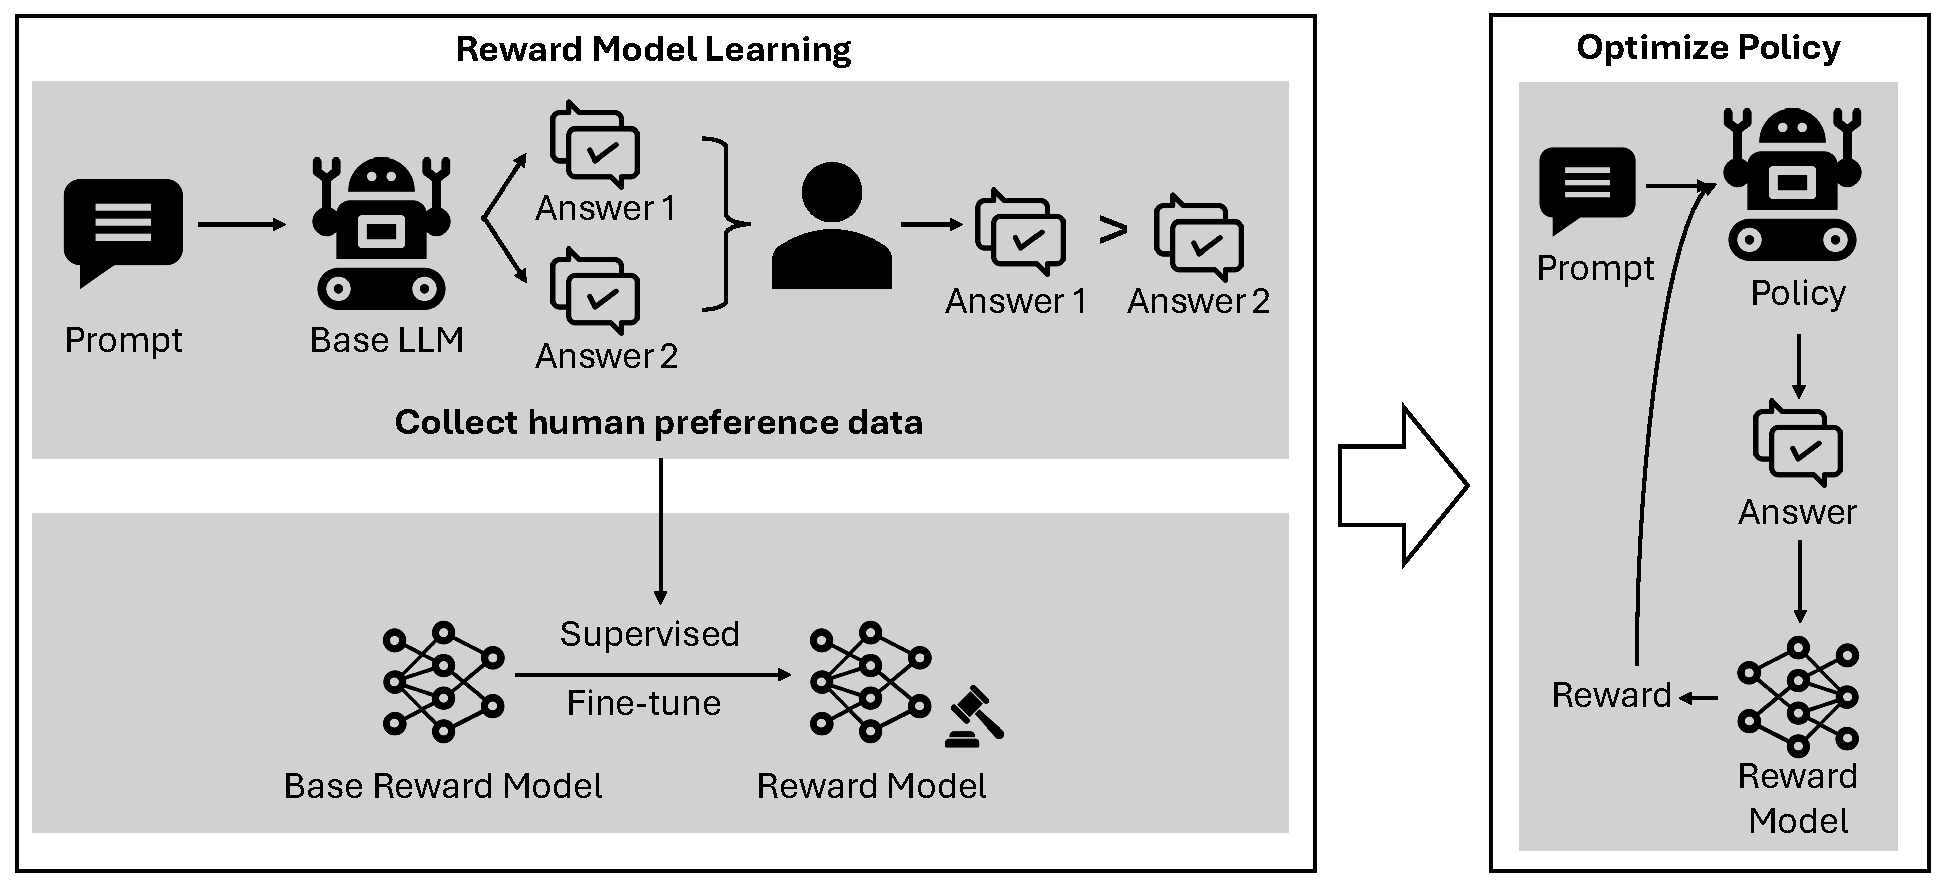
\includegraphics[width=16cm]{figures/figure3.pdf}}
      \caption{Diagram of the RLHF pipeline. On the left, the Reward Model Learning process involves collecting human preference data by comparing answers generated by a base large language model (LLM). The reward model is then fine-tuned based on this data. On the right, the optimized policy is trained using the learned reward model, which guides the agent’s responses to maximize the expected reward.}
  \label{fig:RLHF}
\end{figure}

Reinforcement learning with human feedback (RLHF)\cite{ouyang2022training} replaces manually engineered reward functions with human preferences, which are then used to guide the agent’s learning process. A standard pipeline collects short trajectory segments, queries a human for a preference between two alternatives, fits a reward model so that human-preferred segments receive higher cumulative reward, and then optimizes a policy with the learned reward while continuing to request new comparisons. This loop can align behavior with task intent when reward functions are difficult to specify.

\paragraph{Reward Modeling}
In RLHF, the reward model is trained using human comparisons between two trajectories. For each pair of trajectories $\tau^A$ and $\tau^B$, a human annotator decides which trajectory is preferred. This preference is then used to train a model $r_\phi(s,a)$ to predict the scalar reward for each action-state pair. The reward model loss function is based on cross-entropy and is computed as the difference between the predicted reward of two trajectories. The loss function for the reward model is given by:
\[
\mathcal{L}_{\text{RM}}(\phi) = - \frac{1}{\binom{K}{2}} \mathbb{E}_{x, y_w, y_l \sim \mathcal{D}} \left[ \log \sigma(r_\theta(x, y_w) - r_\theta(x, y_l)) \right],
\]
where $r_\theta(x, y)$ is the scalar output of the reward model for prompt $x$ and response $y$, $y_w$ and $y_l$ are the preferred and less preferred responses, respectively, and $\sigma(\cdot)$ is the logistic sigmoid function.

\paragraph{Reinforcement Learning}
Once the reward model has been trained, it is used to guide the learning of the policy. RLHF applies Proximal Policy Optimization (PPO)\cite{schulman2017proximal} to fine-tune the pre-trained supervised model in a specific environment. In a typical RLHF setup, the environment presents random prompts (such as customer requests) to the agent, which must generate a response. Given the prompt and the agent's response, a reward is generated by the reward model, and the episode concludes.

The primary goal is to maximize the expected cumulative reward, as predicted by the reward model, while ensuring that the policy does not overfit to the reward model. To prevent overfitting, a KL penalty is introduced to control the policy's deviation from the supervised pre-training distribution. The value function is initialized using the reward model and is fine-tuned during the reinfrocement learning phase.

The objective function for RLHF during the policy optimization phase is a combination of the reinforcement learning objective and the supervised pre-training objective. It is given by:
\[
objective(\phi) = \mathbb{E}_{x, y\sim \mathcal{D}_{\pi_{\phi}^{RL}}} \left[ r_\theta(x,y)-\beta\log(\pi_\phi^{RL}(y|x)/\pi^{SFT}(y|x) \right] + \gamma \mathbb{E}_{x\sim \mathcal{D}_{pretrain}}\left[\log(\pi_\phi^{RL}(x) \right],
\]
where $\pi_\phi^{RL}$ is the learned policy, $r_\theta(x, y)$ is the reward predicted by the reward model, and $\beta$ is a hyperparameter controlling the relative importance of the reward signal compared to the policy's prior distribution.

\paragraph{Applications} 
In robotics, RLHF has been applied to enable robots to learn complex tasks from human feedback. In SEED\cite{hiranaka2023primitive}, the authors apply RLHF to teach robots primitive skills using human evaluative feedback. In this setup, a robot learns skills by receiving human feedback, which is used to refine its actions in a simulated environment. The reward model is trained using this feedback, and reinforcement learning is applied to update the robot’s policy based on the learned reward. In FAPL\cite{wang2022feedback} presents an efficient framework for learning socially aware navigation skills for robots using human preferences. This work focuses on reducing the amount of human feedback required by actively selecting which preferences to solicit from human evaluators, minimizing the number of interactions while still enabling the robot to learn complex social behaviors.

While these methods show great promise, they still rely on continuous human feedback, which limits scalability and introduces potential noise in the reward model. RG-VLM, by contrast, removes the need for explicit human involvement by leveraging large vision-language models that generate dense rewards directly from offline data, making it more scalable and efficient for complex tasks.



\section{Reward Design with Vision-Language Model}
Vision-language models (VLMs) align image or video representations with text so that semantically matching pairs lie close in a shared embedding space. A canonical example is CLIP\cite{radford2021learning}, which is trained contrastively on large web-scale image–caption pairs to minimize distance for matching pairs and increase distance for mismatched pairs. This training yields strong zero-shot recognition and text-conditioned scoring without any task-specific fine-tuning. 

BLIP\cite{li2022blip} extends this line by unifying understanding and generation. It bootstraps language supervision from noisy web data with a captioner–filter pipeline, then pretrains models that support image–text retrieval, captioning, and VQA within one framework. Empirically, BLIP\cite{li2022blip} reports state-of-the-art results across these tasks, which indicates stronger cross-modal grounding than contrastive-only training in many settings. This broader capability is attractive for reward design because it can connect visual evidence to natural-language task descriptions more robustly. 

A direct way to turn a VLM into a reward model is to score how well an observation matches a natural-language goal. The method VLM-RMs\cite{rocamonde2023vision} does exactly this with CLIP\cite{radford2021learning}. Given a prompt like “the humanoid is sitting in lotus position,” a per-step reward can be computed as a similarity between the image embedding from the current observation and the text embedding of the prompt, optionally improved by subtracting a baseline prompt that represents the non-goal state. With only a sentence-level description, the authors train agents to perform complex poses and report a clear scaling trend where larger VLMs yield better rewards. 

zero-shot reward from image–text similarity in VLM-RMs\cite{rocamonde2023vision} is simple and powerful, yet it inherits the limitations of general-purpose VLMs. Reported failure modes include limited spatial reasoning, sensitivity to unrealistic or out-of-distribution visuals, and difficulties that grow with task complexity. Per-frame scoring also lacks temporal structure, which hurts credit assignment on long-horizon behaviors and high-dimensional manipulation where intermediate progress may be visually subtle. 
arXiv

RoboCLIP\cite{sontakke2024roboclip} targets the temporal gap by using a pretrained video-and-language model to score entire rollouts. The method embeds a full episode video and a task descriptor that can be either a short text or a single human demonstration video, then uses their similarity as the reward. In practice, RoboCLIP\cite{sontakke2024roboclip} employs S3D\cite{xie2018rethinking}, a video model pretrained with language supervision, to encode the rollout and the descriptor. The reward is issued sparsely at the end of the episode as that similarity score, and the agent is trained with online RL on this signal. RoboCLIP\cite{sontakke2024roboclip} can use in-domain or out-of-domain demonstrations and shows that one demonstration often suffices to drive learning. 

End-of-episode similarity creates a sparse signal in RoboCLIP\cite{sontakke2024roboclip} so exploration and credit assignment can be slow, especially in long-horizon manipulation. Performance depends on domain alignment between pretrained video-language embeddings and the deployment environment. The authors explicitly study alignment and note sensitivity to viewpoint and dataset mismatch, which can bias rewards toward spurious visual cues if the demonstration and rollouts differ in style or context. These issues are amplified when only a single sparse reward is available. 

RG-VLM addresses these gaps by prompting a large vision–language model to produce step-wise, language-conditioned dense rewards on offline trajectories. Dense supervision improves temporal credit assignment for long-horizon tasks. Operating offline avoids cost and risk from online exploration. When desired, RG-VLM can be mixed with sparse task indicators, combining reliable completion signals with Large Vision-Language Model(LVLM) generated dense shaping. In short, RG-VLM keeps the scalability and generality of VLM-based rewards while overcoming the sparsity and temporal myopia that limit zero-shot CLIP\cite{radford2021learning} scoring and video-only end-of-episode rewards.


\section{Reward Design with Large Vision-Language Model}
\begin{figure}[H]
    \centerline{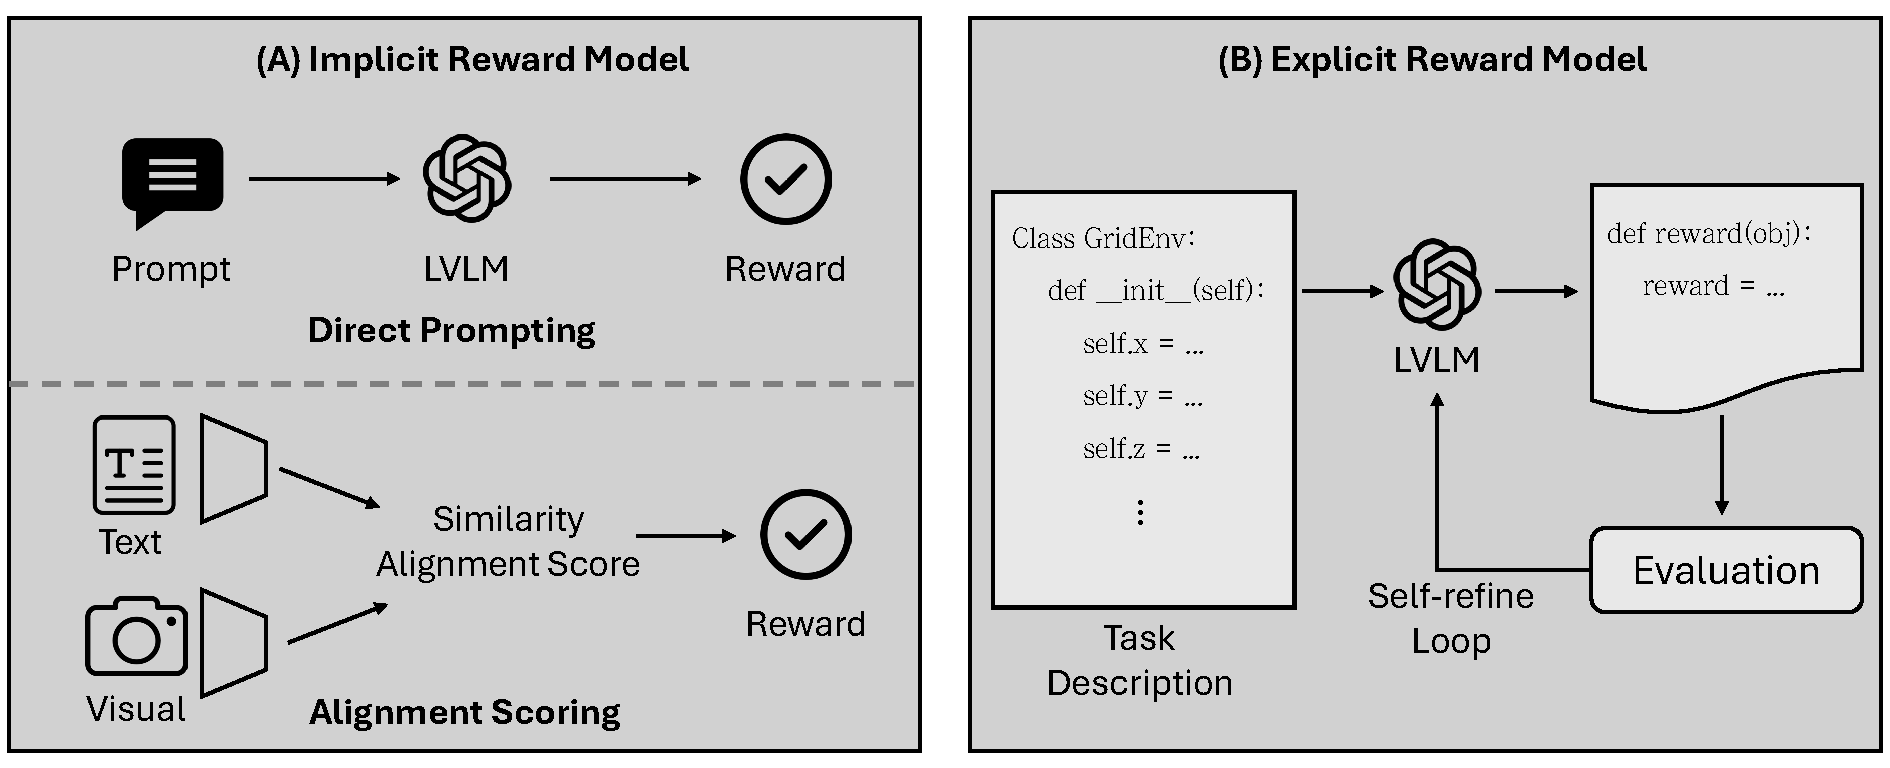
\includegraphics[width=16cm]{figures/figure4.pdf}}
      \caption{Diagram illustrating the two approaches for using LVLMs as reward designers. (A) Implicit Reward Model: LVLMs provide reward signals through direct prompting, where a language prompt is used to evaluate behavior, and alignment scoring, where similarity between text instructions and visual observations is computed. (B) Explicit Reward Model: LVLMs generate executable code for defining reward functions, which can be iteratively refined through a self-refinement loop based on evaluation, allowing for transparent and adaptable reward design.}
  \label{fig:LVLM_reward}
\end{figure}

Designing effective reward functions is both foundational and notoriously difficult in reinforcement learning, especially in complex or real-world settings where the desired behavior cannot be cleanly captured by a single scalar signal\cite{eschmann2021reward}. Classical approaches try to make feedback denser by decomposing a goal into a sequence of subgoals or by adding auxiliary objectives that correlate with long-term success\cite{andreas2017modular, mirchandani2021ella}. These strategies often demand extensive domain expertise and careful engineering, and they are brittle when tasks, sensors, or operating conditions shift\cite{booth2023perils}. Recent progress in large vision-language models reframes this challenge as a dynamic, knowledge-driven design problem that is informed by language, perception, and reasoning rather than a fixed hand-coded specification. Because LVLMs carry broad world knowledge, understand multimodal context, and perform in-context learning and code generation, they can serve as high-level reward designers in two complementary roles. First, as implicit reward models, they infer scalar values directly from observations and natural-language instructions, providing dense supervision even when ground-truth rewards are sparse or undefined. Second, as explicit code generators, they author interpretable and executable reward programs whose logic mirrors the task’s success criteria. In domains like dexterous robotic manipulation, where reward signals are sparse and progress is visually subtle, LVLMs can assess success against linguistic goals or visual affordances through prompting or iterative refinement\cite{ma2023eureka}. By turning task semantics into either stepwise scores or readable code, LVLMs reduce the burden of handcrafted shaping and create a clearer bridge between symbolic task understanding and low-level policy optimization. This perspective lowers the barrier to reward design, improves transparency and flexibility, and points toward more generalizable and human-aligned reinforcement learning systems.

\subsection{Implicit Reward Model}
In many realistic domains, reward specification is difficult because signals are sparse, goals are ambiguous, or success criteria are not directly observable. Large vision–language models provide a scalable alternative by serving as implicit reward models that infer scalar supervision from observations and task descriptions using pretrained knowledge and cross modal grounding. Instead of relying on hand crafted objectives, LVLMs can evaluate the agent’s behavior at the level of a state, a short segment, or an entire trajectory and return a numeric score that functions as auxiliary shaping or as an overall success estimate. The supervision can be episodic or stepwise depending on how context is summarized for the model. It can be applied in online learning to guide exploration or in offline learning to relabel fixed datasets. Because the signal is derived from natural language instructions and visual evidence, the same interface transfers across tasks without redesigning reward code. This high level view establishes the role of LVLMs as implicit reward generators.

\paragraph{Direct Prompting. }
Direct prompting treats a large vision–language model as a surrogate reward function that evaluates behavior from natural language descriptions and a compact snapshot of context. Instead of hand-coding a scalar objective, the designer supplies a short goal description and a small window of observations and actions. The model returns a score or a categorical verdict that is converted into a numeric reward at the step or segment level. In its simplest form, prompting with a few examples of desirable and undesirable behavior together with a concise preference rubric is sufficient to obtain a proxy reward model. This idea shows that carefully written prompts can replace a significant amount of manual shaping and that the interface scales across tasks because goals are written in language rather than code \cite{kwon2023reward}.

Building on this principle, the Read-and-Reward framework\cite{wu2023read} asks an LVLM to read unstructured instruction manuals and extract task-relevant cues before rating the agent’s behavior. A QA extraction module first performs question–answer extraction and summarization to distill rules from documents. A reasoning module then combines those distilled rules with the current observation window and the language goal to issue a scalar assessment. When used as dense feedback, these assessments speed up learning and improve final performance, since the reward reflects task semantics that would otherwise be expensive to encode manually \cite{wu2023read}.

Prompting can also generate auxiliary shaping without hand-crafted subgoals. Given an abstract goal description, a question generation and QA pipeline elicits intermediate objectives from the LVLM. The agent then receives an intrinsic reward that measures progress toward these LVLM-suggested sub-objectives. This additional signal encourages trajectories that systematically recover partial information needed to satisfy the global goal and reduces the burden of manual decomposition \cite{carta2023grounding}.

Continual learning introduces an added difficulty because the agent must retain past knowledge while adapting to new tasks. The Lafite-RL framework\cite{chu2023accelerating} addresses this by producing interactive, stepwise rewards that mimic human feedback. It uses two prompts in tandem. The first summarizes the scene so that the LVLM forms an accurate understanding of context. The second specifies the evaluation criterion so that the model can produce a calibrated score for the current behavior. The resulting supervision accelerates learning while reducing human effort during agent–environment interaction and has been shown to scale across a set of tasks with limited manual supervision \cite{chu2023accelerating}.

From a systems perspective, prompt-based reward estimation benefits from simple calibration layers that convert raw model scores into stable training signals. Designers often apply linear scaling and clipping to keep rewards within useful ranges, perform temporal smoothing to reduce variance across adjacent steps, and aggregate multiple prompt variants to improve robustness. These pragmatic choices make direct prompting a practical tool for generating dense supervision in domains where ground-truth rewards are sparse or very costly to engineer.


\paragraph{Alignment Scoring. }
In visual reinforcement learning, an effective way to realize implicit rewards is to measure how closely the current observation aligns with the goal description in a shared vision–language embedding space. The reward is then defined as a function of this alignment. A common implementation uses a frozen VLM such as CLIP\cite{radford2021learning} to embed the state image and a short natural-language prompt that specifies the goal. Let $f_I(o_t)$ denote the image embedding of the observation at time $t$ and let $f_T(l)$ denote the text embedding of a goal description $l$. Given a candidate set of goals $L$ and a temperature $\tau > 0$, the method computes a softmax probability over goals using cosine similarity. The probability that the agent satisfies goal $l$ at time $t$ is 
$$p_{t,\ell}=
\frac{\exp\!\big(\langle f_I(o_t),\, f_T(\ell)\rangle / \tau\big)}
{\sum_{\ell' \in \mathcal{L}} \exp\!\big(\langle f_I(o_t),\, f_T(\ell')\rangle / \tau\big)}.$$
VLM-RMs\cite{rocamonde2023vision} show that thresholding this probability produces a simple binary reward that needs only a one-sentence prompt and minimal engineering. The binary signal is written as $r_t=1\{p_{t,l}\geq \beta\}$ with a design threshold $\beta$.

Several variants replace the binary signal with a shaped score that preserves more information. A direct choice uses the raw similarity $\langle f_I(o_t), f_T(l)\rangle$. A more robust form subtracts the similarity to a negative description $l_{neg}$ that represents an undesired state. The shaped reward becomes
$$r_t=\langle f_I(o_t),\, f_T(\ell)\rangle-\langle f_I(o_t),\, f_T(\ell_{\text{neg}})\rangle.$$

which reduces spurious rewards when the scene contains distractors that correlate with the goal text.

Alignment scoring is not limited to per-step text goals. Another line labels expert demonstrations by aligning each frame or short segment with a textual task description using a frozen encoder. The labeled scores train an imitation or offline RL policy and help mitigate mis-generalization because the labels reflect semantic similarity rather than brittle hand-coded heuristics \cite{kim2023guide}. This approach also supports segment-level or trajectory-level aggregation using simple statistics such as a moving average or the maximum over a sliding window, which stabilizes training on jittery camera inputs.

Beyond imitation, Language Reward Modulated Pretraining, abbreviated LAMP\cite{adeniji2023language}, uses alignment as a shaped exploration signal that bootstraps sample-efficient learning. The framework computes alignment between image observations and textual instructions using a frozen visual–language encoder such as R3M \cite{nair2022r3m}, feeds the score as a noisy but informative bonus into a visual model-based learner such as the Masked World Model \cite{seo2023masked}, and combines it with a novelty-seeking objective. Images are sourced from Ego4D\cite{grauman2022ego4d} and instructions are produced by a language model. The result is a modular pipeline that improves early exploration without a hand-engineered reward for each task.

A complementary direction uses VLMs to generate preference labels for short behavior pairs conditioned on a text goal\cite{wang2024rl}. The labels train a separate reward model that is then optimized by RL. Experiments on vision manipulation tasks report that preference supervision from VLMs provides a more stable learning signal than regressing raw per-step scores directly. This observation is consistent with the intuition that segment comparisons are easier to judge reliably than instantaneous frame scores.

In summary, alignment scoring turns the representation power of pretrained vision–language encoders into reward signals. The same few lines of code apply across tasks because goals are written in language and observations are embedded by a frozen model. Practitioners often add simple calibration such as temperature tuning, reward clipping, and temporal smoothing. With these additions, alignment scoring delivers practical dense or binary rewards in settings where ground-truth specification is costly or infeasible.

\subsection{Explicit Reward Model}
Large vision–language models(LVLMs) can act not only as critics that score behavior but also as explicit reward designers that generate executable code which computes rewards inside the training loop. This perspective improves transparency because the logic that assigns credit is written as readable code rather than hidden in a black-box score. It also invites systematic improvement. Developers can inspect the program, add safety checks, and iteratively refine it when failure modes appear. Compared with prompt-based shaping or alignment scoring, the explicit route leverages the LVLM’s code generation and symbolic reasoning to construct full reward functions that reference both environmental state and linguistic task specifications.

A first line of work demonstrates that high-level instructions in natural language can be translated into low-level reward terms and weights. The LVLM takes a task description that a human would write and returns code snippets that compute distances, contact conditions, task phase indicators, or penalties. When this code is plugged into a standard RL pipeline, robots execute a broad set of tasks without manual reward engineering. Reports show large gains in task success rates when compared with hand-written baselines, which indicates that the mapping from language intent to programmatic reward logic can close the gap between what humans ask for and what the agent optimizes \cite{yu2023language}.

A second line introduces self-refining reward design. The process begins with an initial generation step that samples several candidate reward programs from the LVLM given the environment API and the task text. Each candidate is compiled and used to train a policy for a short budget. The observed return serves as a score for the underlying reward code. Top candidates are then returned to the LVLM together with short critiques or run-time traces, and the model proposes improved versions. This design–evaluate–reflect loop repeats for multiple rounds. Over time the reward programs become more aligned with the task, and empirical results show that LVLM-designed rewards can rival or surpass carefully engineered baselines \cite{madaan2023self, song2023self}.

The Eureka\cite{ma2023eureka} framework embodies this idea at scale. It uses the environment source code and a natural language task description to prompt a coding model for many reward candidates, trains short-horizon policies under each candidate, ranks candidates by the achieved return, and feeds the best ones back to the model for reflection and revision. Iterating this cycle leads to reward programs that reach or exceed human-level design quality on dexterous manipulation tasks that were previously considered intractable with manual shaping\cite{ma2023eureka}. The key advantage is that the LVLM does not only emit numbers. It emits structure that can be audited, tested, and improved.

A complementary approach, Text2Reward, turns free-form environment descriptions into shaped dense reward programs that are executable. Since reinforcement learning is sensitive to reward design and language can be ambiguous, Text2Reward keeps a human in the loop. The policy trained under the generated reward is executed, human evaluators provide concise corrective feedback, and the LVLM edits the reward code accordingly. This hybrid procedure shows that code-generating LVLMs are useful not only as initial designers but also as adaptable collaborators that incorporate supervision to yield context-specific reward signals \cite{xie2023text2reward}.

From a systems perspective, explicit reward modeling benefits from a few practical conventions. First, the generated code should expose tunable coefficients and units so that calibration is straightforward. Second, the code should be deterministic and side-effect free to make training runs reproducible. Third, safety constraints and rule checks should be encoded near the reward logic to avoid spurious incentives. Finally, evaluation should use fixed training budgets and common random seeds to ensure that the selection of reward programs reflects genuine improvements rather than variance. These practices make explicit LVLM-authored rewards a viable replacement for manual shaping in complex domains.

\subsection{Summarization and Outlook}
Using large vision–language models as reward designers marks a substantive shift in how task objectives are specified and translated into agent behavior. Traditional reward engineering has depended on subgoal decompositions and auxiliary objectives that require domain expertise and painstaking manual tuning. LVLMs provide a language–driven interface that automates much of this process through prompting, alignment scoring, and even code synthesis, while preserving interpretability because prompts, scoring rules, or generated programs make the supervision logic explicit. In practice this paradigm lowers the barrier to deploying RL in complex settings, reduces brittle hand-crafted heuristics, and creates a clearer bridge between high-level task semantics and low-level policy optimization, with encouraging results across diverse domains.

Important limitations remain. Reward functions inherited from LVLMs can carry model and prompt biases that propagate into agent behavior \cite{ferrara2023should}. Most mitigation work has focused on societal or demographic bias \cite{gallegos2024bias}, yet task-specific bias is less studied and can surface as unsafe shortcuts, strategically misaligned behavior, or over-reliance on spurious cues. The risk is heightened in preference-based RL, where policies optimize against learned reward models. If the underlying LVLM or labeling procedure encodes inaccurate preferences, optimization pressure can produce overfitting to flawed reward surrogates and degrade real task performance \cite{gao2023scaling}.

Several remedies help manage these risks while retaining the benefits of LVLM-driven rewards. Reward regularization can incorporate preferences implied by the agent’s value function so that learning resists biased supervision and better approximates the true objective \cite{chakraborty2023rebel}. Human-in-the-loop oversight remains an effective safeguard when an evaluation module allows targeted interventions and corrections whenever policies violate safety rules or deviate from intent. Ensemble strategies that combine outputs from multiple models or prompt variants reduce idiosyncratic errors and average out model-specific biases, which yields more robust and less biased policy behavior \cite{radwan2024addressing}. Alongside these, practical calibration of reward scales, reproducible evaluation protocols, and systematic audits of failure cases are essential to make LVLM-based reward design reliable in deployment.

Future research should improve the alignment, transfer, and controllability of LVLM-designed rewards. For implicit reward models, near-term priorities include reducing ambiguity in instructions, strengthening perceptual grounding, and validating that generated signals track human intent across tasks. Longer-term goals include robust transfer in multi-task and visually rich environments and principled ways to combine implicit signals with sparse environment rewards. For explicit reward models, current limitations stem from reliance on general commonsense knowledge and template-heavy code generation. Short-term progress can come from prompts augmented with structured external knowledge and domain ontologies, as well as from program analysis tools that check units, invariants, and safety constraints. Longer-term efforts should pursue template-free code synthesis, better verification and testing pipelines, and adaptive refinement loops that remain stable under distribution shift. As LVLMs advance in grounding, reasoning, and program synthesis, their integration into the reward pipeline can automate one of RL’s most difficult components, provided that alignment, safety, and cross-domain scalability remain central design objectives.

\chapter{Method}
\begin{figure*}[ht!]
    \centering
    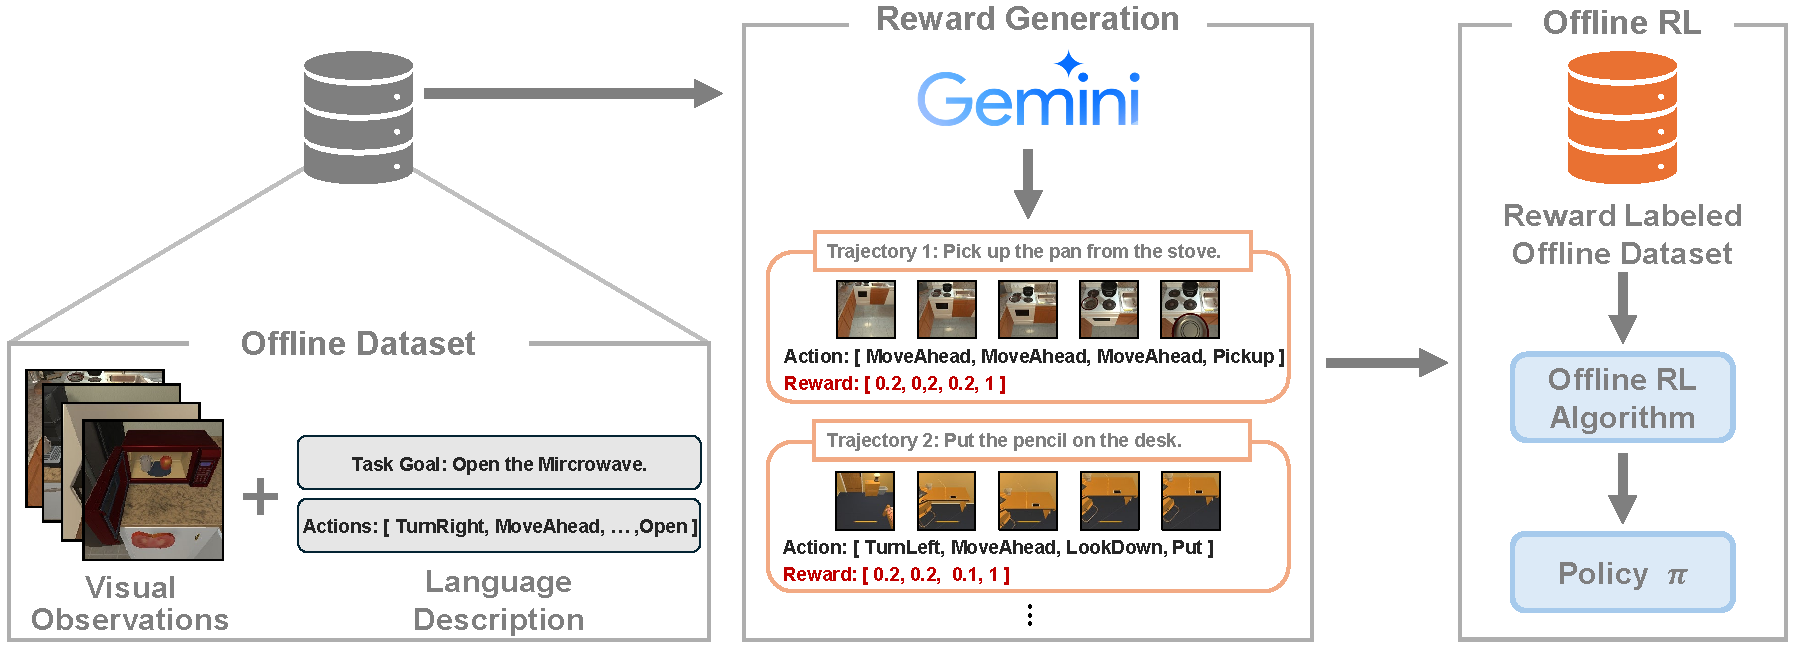
\includegraphics[width=16cm]{figures/figure5.pdf}
    \caption{Overview of the RG-VLM method. The offline dataset, consisting of visual observations and language descriptions (task goals and actions), is fed into the LVLM (Gemini in this case) to generate rewards for each trajectory. The generated rewards are assigned to each action within the trajectory and stored in the reward-labeled offline dataset. This dataset is then used to train the agent’s policy using an offline RL algorithm. The trained policy is optimized based on the reward signals generated by the LVLM.}
    \label{fig:altorithm_flow}
\end{figure*}

In this section, we introduce RG-VLM, a novel method for generating reward signals from offline data using large vision-language models (LVLMs) such as Gemini 1.5 Pro \cite{reid2024gemini}, GPT-4 \cite{achiam2023gpt}, and Flamingo \cite{alayrac2022flamingo}. The goal of RG-VLM is to address the challenge of reward design in reinforcement learning (RL) by using LVLMs to provide a dense, interpretable, and dynamic reward signal based on visual observations, actions, and task goals described in natural language.

Traditional reward function design in RL often relies on manual crafting, decomposing tasks into subgoals, and using expert knowledge. These approaches can be time-consuming and challenging, particularly for complex or real-world environments where tasks may not have easily defined reward functions. RG-VLM offers an alternative by leveraging the power of LVLMs to generate contextual and adaptable rewards from natural language descriptions and visual data. This removes the need for hand-coding complex reward structures and allows for scalable, flexible reward generation that can be applied to a wide range of RL tasks.

RG-VLM operates in two stages to generate rewards from offline data. First, the LVLM analyzes the transitions between observations to understand the agent’s actions and how they contribute to task progression. Then, the LVLM generates a reward for each action, scoring it based on its relevance to the task goal. The generated rewards are used to relabel the offline dataset, and the reward-labeled dataset is subsequently used to train the agent’s policy using any offline RL algorithm.

In the following sections, we will describe the detailed process of reward generation by LVLM in two stages, as well as the offline RL training procedure used to learn the policy from the reward-labeled dataset. We will also discuss the key considerations, such as window size and input prompts, which ensure the efficiency and accuracy of the reward generation process.

\section{Reward Generation by Large Vision-Language Model}
\begin{figure*}[h]
    \centering
    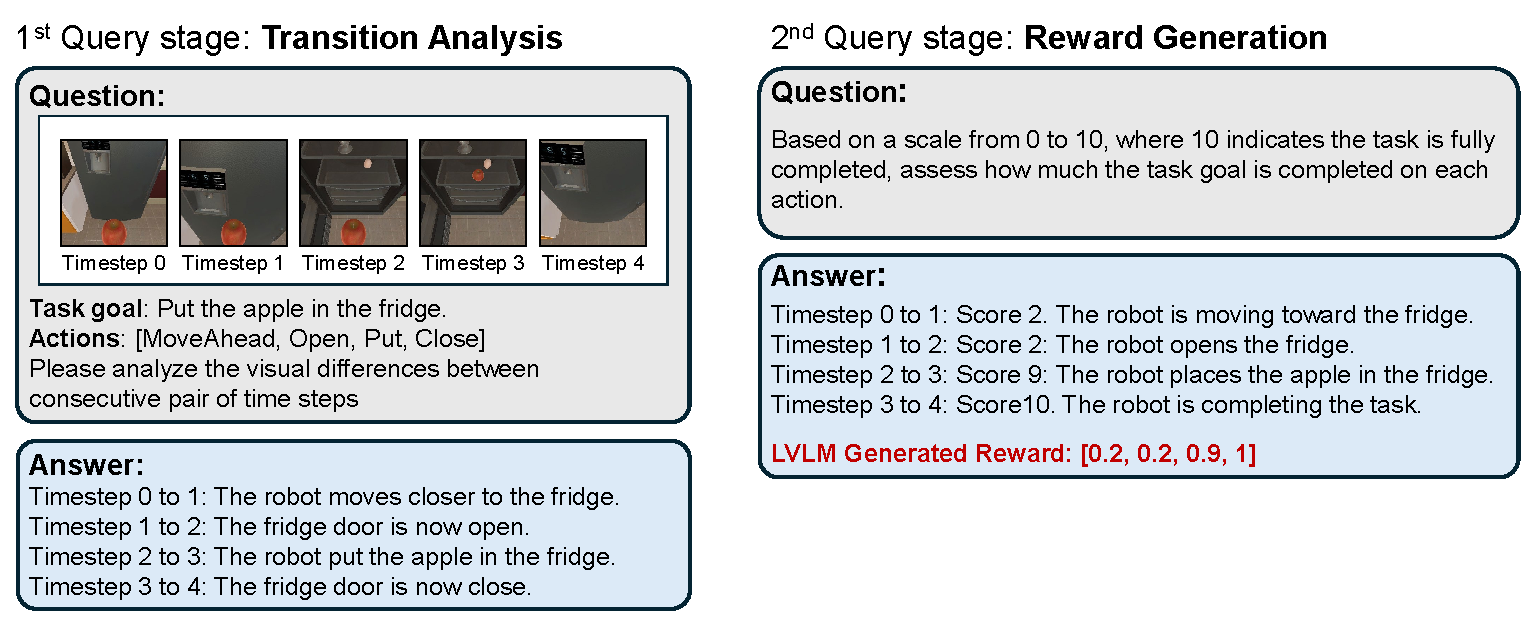
\includegraphics[width=16cm]{figures/figure6.pdf}
    \caption{Example of RG-VLM querying process. The LVLM is queried in two stages. In the first stage, the LVLM analyzes sequences of visual observations, actions, and the task goal to understand how actions affect task progression. In the second stage, the LVLM assigns reward scores (0 to 10) based on each action’s contribution to the task.}
    \label{fig:RG-VLM_reward_generation}
\end{figure*}


The process of reward generation by RG-VLM is carried out in two distinct stages. In this section, we describe each stage in detail, emphasizing the input data, prompt formulation, and the way the LVLM processes and generates rewards for each transition in the offline dataset. Additionally, we discuss the critical design decisions, such as the window size, which helps ensure both computational efficiency and the quality of the reward signals.

\subsection{1st Stage: Transition Analysis with LVLM}
In the first stage of reward generation, RG-VLM processes each trajectory in the offline dataset by analyzing the transitions between consecutive observations. A transition consists of an observation, the action taken by the agent, and the resulting next state. The goal in this stage is to help the LVLM understand the context of the transition—essentially, how each action contributes to progressing toward the task goal.

The input to the LVLM during this stage is a concatenated sequence of visual observations from the environment, paired with the corresponding actions taken by the agent, as well as a description of the task goal, which is provided in natural language. The task goal can be a simple directive like "navigate to the red object" or more complex instructions describing long-term objectives.

Once the observations and actions are concatenated and the goal is formulated into a prompt, the LVLM analyzes the sequence. It compares the visual input at each transition with the task goal described in natural language, helping it recognize which parts of the observation are relevant to the desired outcome and which are not. The LVLM also evaluates the effectiveness of each action in the context of the goal.

The first stage is critical because it allows the LVLM to build an understanding of the agent's behavior and its connection to the overall task. The LVLM doesn’t generate rewards at this point but instead gathers information about the relevance of the actions taken, based on the visual and textual input provided. This understanding sets up the LVLM for the next stage, where it will assign rewards based on this analysis.

\subsection{2nd Stage: Reward Generation with Large Vision-Language Model}
In the second stage, the LVLM is queried again to assign rewards for the actions taken during the transitions. This time, the model outputs a numerical reward for each action, which represents the agent's contribution toward completing the task. The reward is generated on a scale from 0 to 10, with 10 representing full contribution toward achieving the task goal, and 0 indicating no contribution or irrelevant actions.

During this stage, the LVLM leverages its reasoning abilities to evaluate the actions in the context of the task goal. Actions that are directly related to advancing the task receive higher rewards, while actions that don’t contribute meaningfully to the task’s progression are assigned lower rewards. The reasoning capability of LVLMs allows them to take into account not only the current state and action but also the overall progress of the task as described by the goal. By doing so, the model can generate more accurate and interpretable rewards that guide the learning process more effectively.

For example, if the agent is tasked with picking up a red object, actions like moving closer to the object or interacting with it might receive higher rewards, while unrelated actions, such as moving away from the target, would receive lower rewards. The LVLM’s ability to interpret visual and textual cues in tandem allows it to assign rewards based on how much each action contributes to the overall task goal.

\subsection{Input Prompts and Output Rewards}
or both stages of the process, a critical element is the input prompt formulation. In RG-VLM, the task goal and the sequence of visual observations are combined into a single input prompt. This prompt is then fed into the LVLM to guide its analysis and reward generation. The input format is carefully designed to provide the LVLM with enough context to understand the task, the observations, and the agent’s actions.

During the first stage, the input consists of the concatenated observations, actions, and the task goal. The LVLM analyzes the sequence of actions and states and forms an understanding of the transition. In the second stage, the model is asked to assign a reward to each action, which is based on its perceived effectiveness in achieving the goal.

The reward generation process is designed to be scalable and flexible. Once the LVLM generates the rewards, the offline dataset is re-labeled with these new reward signals. The reward-labeled offline dataset is then ready for use in training the RL agent. The next section details how this reward-labeled dataset is used for offline RL training.

\subsection{Window Size and Efficiency Consideration}
The efficiency of the reward generation process in RG-VLM is influenced by the choice of window size. A window refers to the number of transitions that are grouped together for processing by the LVLM. In RG-VLM, the window size is set to 8. For each window, 8 consecutive transitions are collected, and their corresponding visual observations are concatenated into a single image. This window size ensures a balance between computational efficiency and the quality of the reward signals.

However, the window size was not chosen arbitrarily. It was fine-tuned through a testing process to achieve a high accuracy and recall for the sparse rewards assigned during the reward generation. Specifically, sparse rewards are defined as follows: if the agent successfully satisfies the task goal at the end of the trajectory, it receives a reward of 1; otherwise, it receives a reward of 0. The goal is to ensure that the sparse reward signal accurately reflects whether the agent has accomplished its task.

The window size was adjusted such that the accuracy and recall of the sparse reward exceeded 0.85. This testing process ensures that the window size not only improves computational efficiency but also preserves the precision of the sparse reward signal. If the window size is too small, a large number of queries would be required to cover the entire trajectory, leading to increased computational costs and time. On the other hand, if the window size is too large, the concatenated image may become either too large or lose important details when resized, making it difficult for the LVLM to effectively analyze the transitions and assign accurate rewards.

Through preliminary experiments, it was found that a window size of 8 strikes the optimal balance, preserving image quality while minimizing the number of queries needed for each trajectory. This window size not only ensures computational efficiency but also maximizes the accuracy and recall of sparse reward assignments, providing high-quality rewards for the agent’s learning process.

\section{Offline RL Training}
Once the offline dataset has been re-labeled with rewards generated by the large vision-language models (LVLMs), the next step in RG-VLM is to train a reinforcement learning (RL) policy using the reward-labeled data. In this section, we describe the process of using the reward-labeled offline dataset to learn the agent's policy. We also discuss the key components of the offline RL training process, including the selection of RL algorithms, the optimization procedure, and the interaction between the agent’s policy and the reward signals.

\subsection{Offline RL Policy Learning}
The core of RG-VLM's training process is to use the reward-labeled offline dataset for policy optimization. The offline RL setting means that no new environment interaction is required, and the agent must learn solely from the trajectories and the rewards provided by the LVLM-generated signals. This is advantageous in environments where real-time interaction with the environment is costly or impractical.

To train the policy, RG-VLM utilizes any offline RL algorithm that can handle the reward signals generated in the previous steps. Common offline RL algorithms include Implicit Q-Learning (IQL)\cite{kostrikov2021offline}, Conservative Q-Learning (CQL)\cite{kumar2020conservative}, and TD3+BC (Twin Delayed Deep Deterministic Policy Gradient with Behavior Cloning)\cite{fujimoto2021minimalist}. These algorithms can operate with the reward-labeled dataset by optimizing the policy through a series of updates that minimize the discrepancy between the predicted reward and the observed reward.

\subsection{Training Procedure}
The offline RL training procedure follows a standard pipeline for reinforcement learning. First, a policy network $\pi_\theta(a|s)$ is initialized with random weights or a pretrained model, if available. Then, the algorithm iteratively samples trajectories from the reward-labeled offline dataset $D$, where each trajectory consists of state–action pairs and their corresponding rewards. The policy is updated by optimizing a loss function that minimizes the difference between the predicted reward and the reward provided by the LVLM.

For instance, in IQL\cite{kostrikov2021offline}, the loss function involves computing the value estimate of the agent’s actions using a soft value estimator. The policy is then improved based on this estimate, which is done through advantage-weighted regression. The advantage is calculated by subtracting the value of the next state from the current state's value and adjusting the action probabilities accordingly. This ensures that the policy is directed toward actions that provide higher rewards according to the reward model.

The optimization process continues iteratively, refining the policy to maximize the expected return over time. The offline nature of the training means that no online environment interaction is required, reducing the costs and risks associated with exploration in dynamic or dangerous environments.

\subsection{Optimization and Convergence}
The optimization process continues until convergence, which is typically defined by the stabilization of the policy performance or the loss function. The convergence criteria can vary depending on the RL algorithm used, but typically involves checking for minimal changes in the policy over multiple training iterations or when the difference between successive value estimates falls below a threshold.

Throughout training, the reward-labeled offline dataset plays a crucial role in stabilizing the policy learning process. The agent iteratively improves its policy based on the rewards provided by the LVLM, gradually refining its behavior to maximize the expected cumulative reward.

\subsection{Computational Consideration}
Training with offline data offers computational advantages, as there is no need for real-time interaction with the environment. However, the reward generation process itself can be computationally expensive, especially when large-scale LVLMs are involved. The method of reward generation by LVLMs is optimized to ensure that the balance between computational cost and reward accuracy is maintained. By using efficient querying mechanisms and batch processing of trajectories, RG-VLM minimizes the computational cost of reward generation while ensuring high-quality rewards that drive effective policy optimization.

\begin{algorithm}[h]
\small
\caption{RG-VLM: LVLM Reward Generation and Offline RL Training}\label{alg:dr_vlm} 
\begin{algorithmic}[1]
    \STATE \textbf{Input:} A pre-trained LVLM, offline dataset $\mathcal{D}$, window size $w$

    \STATE \textbf{Initialize:} The policy $\pi_{\theta}$
    \STATE \texttt{//RG-VLM: Reward Generation via LVLM}
    \FOR{each trajectory $\tau_i \in \mathcal{D}$}
         \FOR{$t = 1$ to total length $T_{\tau_i}$ with step $w$}

            \STATE Extract samples $\{(s_j, a_j, s_{j+1})_{j=t}^{t+w-1}\}$
            \STATE Concatenate $\{s_j\}_{j=t}^{t+w}$ into an image $\hat{s}$
            \STATE Formulate prompt with $\hat{s}$, $\{a_j\}_{j=t}^{t+w-1}$ and goal $g$
            \STATE Query LVLM to analyze transitions 
            \STATE Query LVLM again to get rewards $\{\hat{r}_j\}_{j=t}^{t+w-1}$

            \STATE Store $\{\hat{r}_j\}_{j=t}^{t+w-1}$ into $\mathcal{D}$
        \ENDFOR
    \ENDFOR

    \STATE \texttt{//Offline RL Policy Training}
    \WHILE{not converged}
        \STATE Sample relabeled trajectories from $\mathcal{D}$
        \STATE Train the policy $\pi$ using an offline RL algorithm 
    \ENDWHILE
\end{algorithmic}
\end{algorithm}
\setlength{\textfloatsep}{0.1in}
In summary, RG-VLM provides a novel method for offline reinforcement learning (RL) by generating rewards from visual observations and task goals using large vision-language models (LVLMs). The process begins with the reward generation phase, where the LVLM analyzes transitions between observations and actions in two stages. In the first stage, the LVLM processes the transitions, understands the relevance of actions to the task goal, and forms an understanding of the task context. In the second stage, the LVLM assigns a numerical reward for each action based on its contribution to achieving the task goal, with a reward scale from 0 to 10.

The reward-labeled offline dataset is then used to train the agent’s policy using any offline RL algorithm, such as Implicit Q-Learning (IQL)\cite{kostrikov2021offline} or Conservative Q-Learning (CQL)\cite{kumar2020conservative}. The RL policy is optimized iteratively by minimizing the difference between the predicted reward and the LVLM-generated reward. The window size, set to 8 in this method, plays a crucial role in balancing computational efficiency and the accuracy of sparse reward assignments. The window size was optimized to ensure a high accuracy and recall for sparse rewards, which are crucial for evaluating the success of the agent’s actions based on task completion.

By using RG-VLM, the process of reward generation becomes efficient, scalable, and flexible. The offline RL setup allows for the agent to learn solely from the historical trajectories without requiring real-time interaction with the environment, which is particularly beneficial for tasks where exploration may be costly or impractical. This method provides a promising framework for enhancing the efficiency of reinforcement learning systems and simplifying reward function design.


\chapter{Experiments}
In this section, we empirically evaluate RG-VLM in a goal-conditioned offline reinforcement learning setting built on the ALFRED benchmark. The main objective of our experiments is to assess whether rewards generated by large vision–language models can serve as effective supervision signals for offline RL, especially in long-horizon, language-conditioned manipulation and navigation tasks. We focus on settings where collecting online interaction is costly and where only a fixed set of trajectories and sparse success labels are available.

We structure our evaluation around three main questions. First, we examine whether RG-VLM can improve policy performance compared to conventional offline RL with only sparse rewards and existing VLM-based reward models, including CLIP-style VLM-RMs\cite{rocamonde2023vision}, BLIP-2\cite{li2022blip} based rewards, and RoboCLIP\cite{sontakke2024roboclip}. Second, we investigate the robustness and generalization of RG-VLM under different initial conditions by comparing performance in fixed start position settings and more challenging random start position settings, which better reflect realistic deployment scenarios. Third, we conduct ablation studies to analyze the contribution of RG-VLM as an auxiliary reward signal on top of sparse rewards and to understand how different LVLM backbones, such as Gemini Pro\cite{reid2024gemini} and Qwen2-VL 72B, affect reward quality and downstream policy learning.

Across all experiments, we use Implicit Q-learning (IQL)\cite{wang2023implicit} as the underlying offline RL algorithm and train policies on reward-labeled offline datasets generated by RG-VLM. We evaluate the learned policies using standard ALFRED metrics such as task success and task completion ratio over varying task horizons. The following subsections describe the experimental setting in detail, present quantitative and qualitative results, and provide ablation analyses that clarify the design choices in RG-VLM.

\section{Experiment Setup}
\subsection{Environment and Tasks}
We conduct our experiments in the ALFRED\cite{shridhar2020alfred} environment, a language-conditioned, long-horizon instruction following benchmark built on a household simulation domain. In ALFRED\cite{shridhar2020alfred}, an agent operates in realistic indoor scenes and is required to complete everyday tasks such as picking up, placing, cleaning, heating, or cooling objects according to high-level natural language instructions. Each task is decomposed into a sequence of lower-level skills that the agent must execute in the correct order, which makes the benchmark particularly suitable for studying long-horizon decision making and multi-step reasoning in reinforcement learning.

For training and evaluation, we follow the data preprocessing protocol introduced in prior work on ALFRED skill learning\cite{zhang2024sprint}. The original ALFRED\cite{shridhar2020alfred} training set contains approximately 6.6k expert trajectories collected by an optimal planner over seven high-level task families with randomly sampled object instances. Each trajectory is annotated with at least three independent sets of natural language instructions and is further segmented into a sequence of 3 to 19 skills, where each skill corresponds to a semantically meaningful subtask. This yields about 141k language-annotated skill trajectories in total. However, a large fraction of these skills correspond to fine-grained navigation behaviors, such as “turn left, look up, and walk to the counter,” which are overrepresented compared to higher-level manipulation skills. To obtain a more balanced skill dataset, navigation-only skills are merged with the immediately following skill, and only the annotation of the next skill is retained. After this consolidation step, the resulting dataset consists of approximately 73k language-annotated primitive skill trajectories. On average, each full trajectory contains about 3.5 skills and each skill consists of roughly 14.3 low-level actions.

RG-VLM is trained on this processed set of 73k primitive skill trajectories, which we treat as an offline dataset of state, action, and language instruction triples. Our choice of ALFRED is motivated by its scale and diversity. The training set spans 120 different scenes, and the evaluation set covers 65 scenes, including unseen scene–instruction combinations. The action space in this domain is also relatively large. The agent can choose among 12 discrete actions, such as moving, looking, picking up, placing, opening, and closing, and interact with 82 different object types. This combination of a rich action space, diverse scenes, and long-horizon tasks makes ALFRED a challenging benchmark for both offline RL and reward modeling.

For evaluation, we adopt the long-horizon task setting derived from the ALFRED dataset to focus on multi-step task composition. Concretely, we evaluate on 100 tasks constructed from ALFRED trajectories, with task lengths ranging from 1 to 6 subtasks. Each evaluation task is specified by a single high-level natural language instruction and requires the agent to successfully execute a sequence of primitive skills to complete the goal. These evaluation tasks are designed to be representative of the original ALFRED benchmark in terms of task composition, scene diversity, and instruction complexity, while allowing controlled analysis across different task lengths.

During evaluation, we consider two initialization regimes. In the fixed initial state setting, the agent is initialized in the same state as in the corresponding offline trajectory, which matches the distribution seen during reward generation and policy training. In the randomized initial state setting, the agent’s initial position is randomized within the same scene, so that the starting state differs from the offline dataset. This random initialization setup is used to assess the generalization and robustness of the learned policies to distributional shifts in the initial conditions. In both settings, the agent receives a sparse reward of 1 only when it successfully completes the task goal, and 0 otherwise. We report task success rate as well as the proportion of the task successfully completed, measured in terms of achieved subtasks. These sparse success signals are also used as a reference when tuning the RG-VLM reward generation process, for example when selecting the window size to achieve high accuracy and recall with respect to final task success.

\subsection{Offline Dataset and Traejctory Collection}
We adopt the preprocessed ALFRED skill dataset described in Section 5.1.1 as the offline dataset for both reward generation and policy learning. In our setting, the offline dataset is treated as a fixed collection of trajectories without any further environment interaction during training, consistent with the offline RL formulation in Section 2.1. Concretely, we denote the offline dataset by $\mathcal{D}_{off}$, which consists of $N$ tajectories:
\begin{equation}
    \mathcal{D}_{\text{off}} = \{\tau_i\}_{i=1}^N,
\end{equation}
where each trajectory $\tau_i$ is a sequence of low-level transitions paired with a language instruction:
\begin{equation}
    \tau_i = \bigl( (s_0, a_0, s_1), (s_1, a_1, s_2), \dots, (s_{T_i-1}, a_{T_i-1}, s_{T_i}), \; l_i \bigr).
\end{equation}

Here, $s_t$ denotes the visual observation at time step $t$ (an RGB egocentric image), $a_t$ is one of the 12 discrete actions available in the ALFRED environment, $s_{t+1}$ is the next state, and $l_i$ is the natural language instruction associated with the corresponding primitive skill or composed task.

The trajectories in $\mathcal{D}_{\text{off}}$ are derived from expert demonstrations generated by an optimal planner in ALFRED\cite{shridhar2020alfred}. The original training set contains approximately 6.6k full task trajectories spanning seven high-level task families. Each full trajectory is segmented into 3--19 skills and annotated with multiple language instructions, yielding about 141k language-annotated skill trajectories in total\cite{srivastava2022sprint}. However, a large fraction of these skills correspond to fine-grained navigation behaviors, which are overrepresented compared to higher-level manipulation skills. To obtain a more balanced skill dataset, navigation-only skills are merged with the immediately following skill, and only the annotation of the latter is retained. After this consolidation step, the resulting dataset consists of approximately 73k language-annotated primitive skill trajectories. On average, each full trajectory contains about 3.5 skills, and each primitive skill consists of roughly 14.3 low-level actions.

From the viewpoint of offline RL, we treat each primitive skill trajectory as an independent episode. For each trajectory $\tau_i$, we construct a sequence of transition tuples
\begin{equation}
    (s_t, a_t, r^{\text{sparse}}_t, s_{t+1}, l_i),
\end{equation}
where $r^{\text{sparse}}_t$ denotes the sparse environment reward. In our setting, the sparse reward is defined at the task level: if the agent successfully completes the task goal (i.e., satisfies all required subtasks for the corresponding ALFRED trajectory), it receives a reward of $1$ at the end of the episode and $0$ otherwise. During training, this sparse signal is available as a reference label but is intentionally too coarse to provide dense guidance at the action level. We therefore regard the dense per-step reward as unobserved and instead rely on RG-VLM to infer it from visual observations, actions, and the language goal.

The same pool of 73k skill trajectories is used across all compared methods, including IQL with sparse rewards only, CLIP-based VLM reward models\cite{rocamonde2023vision}, BLIP-2\cite{li2022blip} based rewards, RoboCLIP\cite{sontakke2024roboclip}, and our proposed RG-VLM. This ensures that any performance differences can be attributed to the quality of the reward signal rather than differences in data coverage. For evaluation, we additionally construct 100 long-horizon tasks of length 1 to 6 subtasks from the ALFRED dataset. These evaluation tasks are not used for training the reward models or policies, and thus serve as held-out tasks for zero-shot or offline generalization.

Finally, we emphasize that the offline dataset remains fixed throughout the entire pipeline: we do not perform any additional data collection or online interaction. RG-VLM operates purely on this static dataset, first generating dense rewards for each transition and then enabling an offline RL algorithm (IQL in our case) to learn a policy from the reward-labeled trajectories. This strict offline setting highlights the importance of high-quality reward generation and provides a realistic testbed for studying LVLM-based reward models in complex, long-horizon, language-conditioned environments.

\subsection{Reward Generation with RG-VLM}
In all experiments, the first step is to convert the language annotated trajectories from ALFRED into dense reward labeled data using RG-VLM. Given the offline dataset of 73k skill trajectories, each paired with a high level natural language instruction, RG-VLM is applied once in an entirely offline manner to generate a scalar reward for every state action transition in the dataset. Concretely, for each trajectory we follow the procedure described in the method chapter and Algorithm 1. The sequence of visual observations, the corresponding low level actions, and the high level task goal are provided as input to a pre trained Large Vision Language Model. Unless otherwise stated, we use Gemini 1.5 Pro as the LVLM for all main experiments, since it showed the most reliable reasoning and reward generation performance on our manipulation tasks. 

To query the LVLM in a way that is both efficient and informative, we segment each trajectory into non overlapping windows of fixed length. For a window size $w=8$, we collect eight consecutive transitions $(s_t, a_t, s_{t+1}), ..., (s_{t+w-1}, s_{t+w-1}, s_{t+w})$ and concatenate the corresponding visual observations into a single grid image. The list of discrete actions in the window and the high level language instruction for the task are then provided as text input. As in the method section, we use a two stage querying scheme. In the first stage, the LVLM is prompted to describe the visual differences between consecutive frames and to reason about how each action changes the environment with respect to the task goal. In the second stage, we query the model again with the same context and instruct it to assign a numerical score to each action that reflects the degree to which the overall task is completed after that step. The LVLM outputs one scalar per action on a scale from 0 to 10, where 10 denotes that the task is fully completed. This two turn interaction encourages the model to first build an explicit understanding of the transitions, which leads to more coherent and interpretable reward assignments in the second stage.

The raw scores produced by the LVLM are then converted into dense rewards that can be consumed by an offline RL algorithm. For each window, we parse the LVLM output into a list of numeric scores and normalize them to the range $[0,1]$ by simple rescaling, so that 0 indicates no contribution to the task and 1 corresponds to full completion. These normalized scores are treated as per step rewards and are attached back to the original transitions in the offline dataset, resulting in a reward labeled dataset $\hat{\mathcal{D}}$. n practice, we fix the window size to 8 based on preliminary experiments. If the window size is too small, the number of LVLM queries explodes and the computational cost becomes prohibitive. If the window is too large, the concatenated image either exceeds the LVLM input resolution or loses important visual detail when resized, which degrades reward quality. We therefore sweep the window size and select $w=8$, which offers a good trade off between efficiency and accuracy, and achieves sparse reward accuracy and recall above 0.85 when we aggregate the LVLM scores into a binary task success prediction and compare it to the environment’s sparse success label. The offline RL algorithm described in the next subsection is then trained on this relabeled dataset, optionally combined with an additional sparse reward on the final state.

\subsection{Offline RL Algorithm and Hyperparameters}
For all experiments, the underlying offline reinforcement learning algorithm is language-conditioned Implicit Q-learning (IQL), as introduced in Section 2.2. The choice of IQL is motivated by its robustness to distributional shift in purely offline settings and its ability to avoid querying out-of-distribution actions by replacing the max operator in the Bellman backup with expectile regression. In our setup, the agent receives both the current visual observation and the natural language instruction as input and learns a language-conditioned policy that predicts low-level actions from this multimodal representation. The RG-VLM reward model only affects the reward labels used for training. The architecture and optimization procedure of the offline RL agent are kept fixed across all experimental conditions in order to isolate the effect of different reward designs.

\begin{table}[t]
\centering
\begin{tabular}{ll}
\toprule
Param & Value \\
\midrule
Batch size & 64 \\
\# Training epochs & 100 \\
Learning rate & $5 \times 10^{-4}$ \\
Optimizer & AdamW \\
Weight decay & 0.1 \\
Discount $\gamma$ & 0.99 \\
Q update Polyak averaging coefficient & 0.005 \\
Policy and Q update period & 1 / train iter \\
Nonlinearity & LeakyReLU(0.2) \\
IQL advantage clipping & [0, 100] \\
IQL advantage inverse temperature $\beta$ & 5 \\
IQL expectile parameter $\tau$ & 0.8 \\
Action chunking length & 15 \\
\bottomrule
\end{tabular}
\caption{Hyperparameters for the language-conditioned IQL policy used in all experiments.}
\label{tab:iql_hyperparams}
\end{table}

In all experiments, we use a single set of hyperparameters for the language conditioned IQL agent and keep this configuration fixed across all reward variants. The settings are largely based on prior work on ALFRED skill learning. We use a batch size of 64, and we train the agent for 100 epochs over the offline dataset instead of using a fixed number of training batches. Mini batches of size 64 are sampled uniformly from the relabeled dataset of 73k skill trajectories, and one gradient update is performed per batch. The learning rate is set to $5e-4$ with the AdamW optimizer and weight decay 0.1. The discount factor is fixed to $\gamma=0.99$. The Q target network is updated using Polyak averaging with a coefficient of 0.005 at every training iteration, and both the policy and Q networks are updated once per training step. All networks use LeakyReLU with negative slope 0.2 as the nonlinearity. For IQL specific hyperparameters, we clip the estimated advantages to the range $[0,100]$, set the inverse temperature in the advantage weighted regression objective to $\beta=5$, and use an expectile parameter $\tau=0.8$. All hyperparameters are shared across all methods and experiments, which allows us to attribute performance differences to the reward design rather than to changes in optimization.

\subsection{Baselines and Evaluation Metrics}
To assess the effectiveness of RG-VLM, we compare it against several baselines that represent standard practices in offline reinforcement learning and recent approaches that use vision–language models for reward design. All methods are trained on the same offline ALFRED dataset described in Sections 5.1.1 and 5.1.2, and they share the identical IQL architecture and hyperparameters given in Section 5.1.4. Therefore, any differences in performance can be attributed to the reward signal rather than to changes in the policy learning algorithm.

As a primary offline RL baseline, we use IQL with sparse rewards only. In this setting, the agent receives a reward of 1 at the end of an episode if it successfully completes the ALFRED task and 0 otherwise. No intermediate rewards are provided during the trajectory. This baseline represents the standard offline RL formulation in long-horizon environments where only task success is observed and highlights the difficulty of learning from extremely sparse feedback.

We also include a CLIP\cite{radford2021learning} based zero shot reward model baseline, denoted VLM-RM\cite{rocamonde2023vision}. In VLM-RM, a pre trained vision language encoder computes similarity between the current observation and a text description of the goal. At each step, the visual state is embedded by the image encoder and compared to the embedding of the language instruction. The cosine similarity is converted into a probability over candidate goals by a softmax with temperature, and a binary reward is given when this probability exceeds a threshold. The resulting reward is then used to train IQL\cite{wang2023implicit}. This baseline reflects a widely studied approach in which the VLM directly defines the reward function through alignment scoring.

To examine the effect of stronger vision language encoders, we introduce a BLIP2\cite{li2022blip} based reward baseline. Here, the CLIP\cite{radford2021learning} encoder in VLM-RM is replaced with a BLIP2\cite{li2022blip} vision language model, which provides improved multimodal representations. The basic reward computation remains the same. We embed the current image and the language goal using BLIP2\cite{li2022blip} and transform their similarity into a scalar score that is thresholded to produce step wise rewards. This baseline allows us to disentangle the impact of the LVLM architecture from the design of RG-VLM itself.

Another baseline is RoboCLIP\cite{sontakke2024roboclip}, which uses a pre trained video and language model (S3D\cite{xie2018rethinking}) as a trajectory level reward model. For each trajectory, RoboCLIP\cite{sontakke2024roboclip} compares the video of the agent’s behavior to a single demonstration or language description and outputs a scalar that represents how well the behavior matches the reference. We treat this trajectory level score as a sparse reward that is assigned at the end of the episode and propagate it uniformly to all transitions when training IQL\cite{wang2023implicit}. This baseline tests whether trajectory level alignment alone is sufficient to support robust offline policy learning in ALFRED.

Our main method, RG-VLM, is evaluated in two configurations. In the first configuration, IQL is trained only on the dense per step rewards generated by RG-VLM, without using any environment sparse reward. In the second configuration, RG-VLM rewards are combined with the original sparse success signal. The dense LVLM based reward then serves as an auxiliary shaping signal, while the sparse reward preserves the original task objective. This second configuration is used in the ablation study in order to analyze the role of RG-VLM as an auxiliary reward.

All methods are evaluated on the same set of 100 held out tasks, which are grouped by task length from 1 to 6 subtasks. For each task, the agent is rolled out in the simulator either from the fixed initial state that matches the offline dataset or from a randomized initial position within the same scene. We measure two main metrics. The first is task success rate, defined as the fraction of evaluation tasks for which the agent completes all required subtasks within the time limit. The second is task completion proportion, defined as the fraction of subtasks in a task that are successfully completed. For example, if a task consists of four subtasks and the agent completes three of them, the completion proportion for that episode is 0.75. This metric is equivalent to the normalized return when the sparse subtask reward is 1 for each completed subtask and 0 otherwise.

All methods are trained with five different random seeds. During evaluation, we report the mean and standard deviation of both metrics across seeds. For the plots that show performance as a function of task length, we average the completion proportion over all tasks of a given length and all seeds. These metrics provide complementary views of performance. The success rate captures strict end to end task completion, while the completion proportion reveals partial progress on long horizon tasks and is particularly informative when the agent fails near the end of a complex instruction.

\section{Experiment Results}
In this section, we present empirical results evaluating RG-VLM on the ALFRED benchmark under the offline RL setting described in Section 5.1. Our analysis focuses on three main questions: (1) whether LVLM-generated dense rewards enable better policy learning than conventional sparse rewards and existing VLM-based reward models and (2) how well RG-VLM scales to long-horizon tasks with multiple subtasks and to different initial state configurations. To answer these questions, we compare RG-VLM against IQL with sparse rewards only, CLIP-based VLM-RMs, BLIP2-based reward models, and RoboCLIP, using a shared offline dataset and identical IQL hyperparameters across all methods.

\subsection{Fixed initialization state Results}
\begin{figure*}[h]
    \centering
    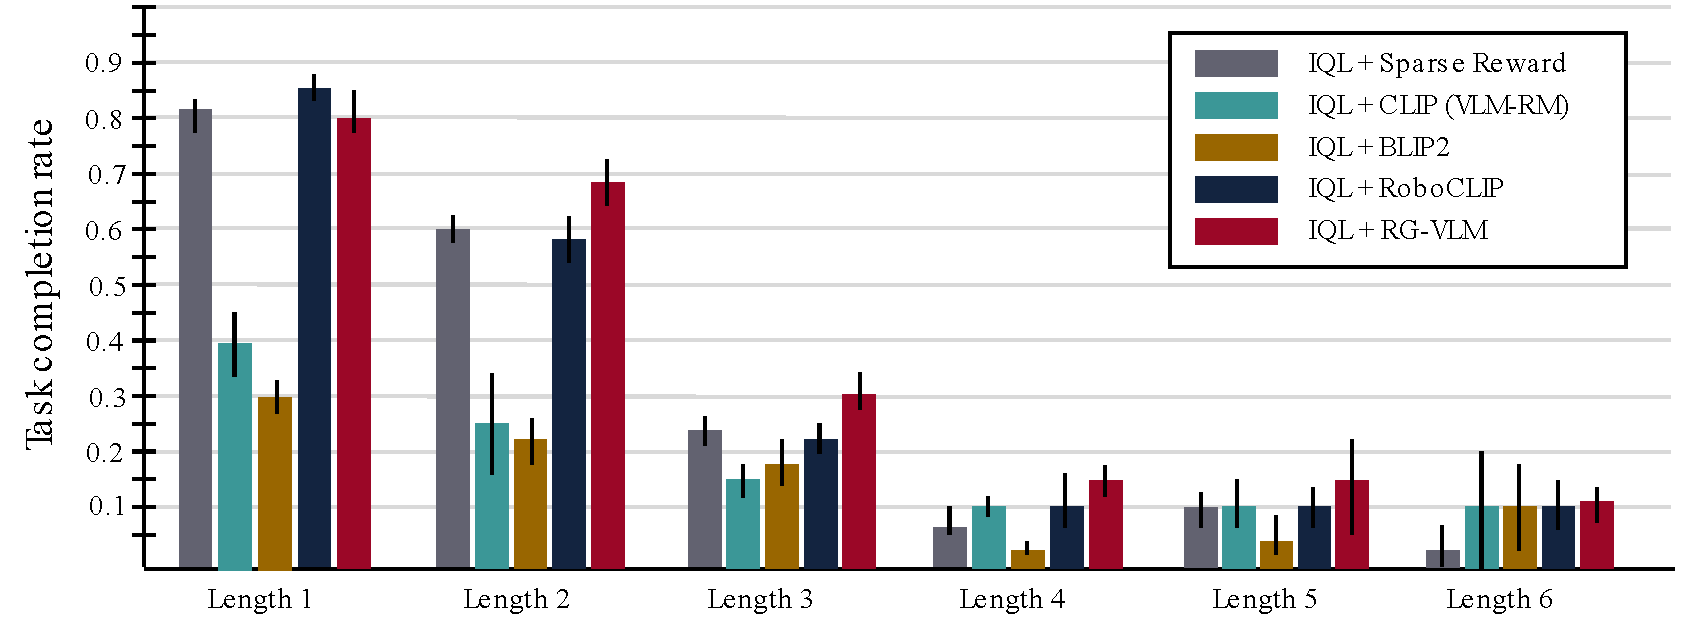
\includegraphics[width=16cm]{figures/figure7.pdf}
    \caption{Task completion rate on ALFRED for different instruction lengths (Length 1–6) under the fixed initial state setting. We compare IQL with sparse reward, CLIP (VLM-RM), BLIP2, RoboCLIP, and RG-VLM rewards; error bars indicate standard deviation over 5 random seeds.}
    \label{fig:exp_result_fixed}
\end{figure*}
In the fixed initialization setting, the agent always starts from the same initial configuration as in the offline trajectories. Figure \ref{fig:exp_result_fixed} reports the proportion of task completed for task lengths from 1 to 6 subtasks.

For length-1 tasks, IQL with sparse rewards already achieves a high completion proportion of around 0.85, reflecting that one-step goals are relatively easy when the start state matches the demonstrations. CLIP- and BLIP2-based rewards perform noticeably worse (around 0.30–0.40), suggesting that single-frame similarity is not sufficient even in this simple case. RoboCLIP and our method (IQL + RG-VLM) both reach around 0.88, clearly outperforming CLIP and BLIP2 and matching or slightly exceeding the sparse-only baseline.

For length-2 tasks, the gap between reward designs becomes more pronounced. IQL with sparse rewards drops to about 0.60, while CLIP and BLIP2 fall to roughly 0.25. RoboCLIP attains a completion proportion close to 0.58, but RG-VLM achieves the highest performance, around 0.68. This indicates that dense, transition-aware rewards help the policy better chain two primitive skills, even when the environment state distribution is favorable.

For length-3 tasks, all methods degrade as the horizon grows, but RG-VLM remains clearly ahead. Sparse-only IQL, BLIP2, and RoboCLIP cluster around 0.20–0.23, while CLIP lags behind near 0.13. In contrast, IQL + Sparse + RG-VLM reaches about 0.30, corresponding to roughly 30\% of subtasks completed on average. This shows that RG-VLM provides more informative intermediate feedback as the number of required skill compositions increases.

For length-4 tasks, the problem becomes substantially more difficult and the completion proportion drops below 0.15 for all methods. Sparse-only IQL falls to roughly 0.08. CLIP and RoboCLIP achieve around 0.12 and 0.11, respectively, and BLIP2 remains lower at about 0.05. RG-VLM attains the highest performance, around 0.13–0.14, maintaining a consistent margin over the baselines despite the increased horizon.

For length-5 tasks, all methods operate in a very low-return regime, with completion proportions roughly between 0.05 and 0.14. CLIP, BLIP2, and sparse IQL are all around 0.05–0.10, while RoboCLIP and RG-VLM reach about 0.11 and 0.14, respectively. Even in these long-horizon settings, RG-VLM provides the most constructive training signal, leading to the best overall performance.

Finally, for length-6 tasks, which are the most challenging in our evaluation, every method achieves less than 0.15 completion proportion. Sparse-only IQL is the weakest, at around 0.05. CLIP and BLIP2 improve to roughly 0.10, and RoboCLIP slightly exceeds them at about 0.11–0.12. RG-VLM is again among the top performers, with a completion proportion around 0.12. Overall, across lengths 1–6, IQL + RG-VLM either matches or surpasses the strongest baseline at each horizon, with especially clear gains once the task length exceeds two subtasks.

\subsection{Random initialization state Results}
\begin{figure*}[h]
    \centering
    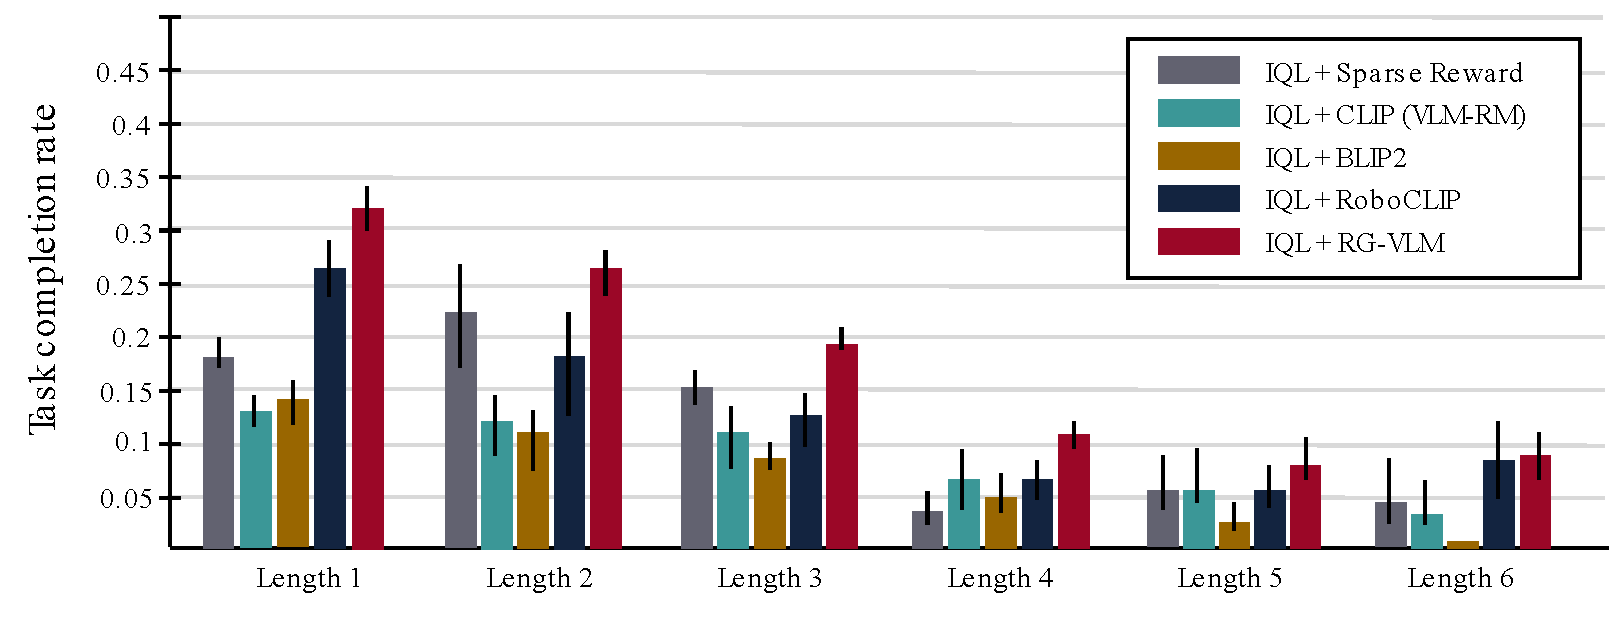
\includegraphics[width=16cm]{figures/figure8.pdf}
    \caption{Task completion rate on ALFRED for different instruction lengths (Length 1–6) under the random initial state setting. We compare IQL trained with sparse reward, CLIP (VLM-RM), BLIP2, RoboCLIP, and our RG-VLM reward models. While all methods suffer a noticeable performance drop compared to the fixed initial state, IQL + RG-VLM consistently achieves the highest success rate across all lengths, indicating that the proposed reward model provides better generalization and robustness to changes in the initial state.}
    \label{fig:exp_result_random}
\end{figure*}
The randomized initialization setting is more challenging, since the agent starts from a random position in the same scene rather than from the demonstration initial state. This introduces a distribution shift between training and evaluation. Figure \ref{fig:exp_result_random} shows the proportion of task completed across task lengths from 1 to 6.

For length-1 tasks, all methods experience a noticeable drop compared to the fixed initialization case. IQL with sparse rewards decreases from roughly 0.85 to about 0.18. CLIP and BLIP2 lie around 0.12–0.13, and RoboCLIP achieves about 0.26. RG-VLM attains the highest completion proportion, around 0.32, which corresponds to an improvement of roughly 77\% over the sparse baseline in this setting.

For length-2 tasks, the pattern is similar but the ranking between methods becomes clearer. Sparse IQL remains relatively strong at about 0.23, reflecting that short-horizon tasks can still sometimes be solved from new starting positions. CLIP and BLIP2 are again lower, near 0.11–0.13, while RoboCLIP reaches around 0.19. RG-VLM continues to perform best, with a completion proportion around 0.26, surpassing both sparse rewards and all VLM-based baselines.

For length-3 tasks, all scores drop further, indicating the difficulty of composing three skills from unfamiliar initial poses. Sparse IQL, CLIP, BLIP2, and RoboCLIP cluster between roughly 0.10 and 0.16, with none of them clearly dominating across all seeds. In contrast, RG-VLM achieves about 0.19, maintaining a clear margin over the other methods and showing that its dense rewards still guide the agent toward meaningful partial progress even when the start state differs from the demonstrations.

For length-4 tasks, the completion proportion becomes very small for every method. Sparse IQL drops to around 0.04, BLIP2 to roughly 0.05, and CLIP and RoboCLIP to around 0.08 and 0.07, respectively. RG-VLM nonetheless reaches about 0.10, which, although numerically small, still represents a consistent improvement over all baselines in a regime where solving the full task is extremely challenging.

For length-5 tasks, the returns remain low, but the relative ordering between methods is stable. BLIP2 nearly collapses, with a completion proportion around 0.02. Sparse IQL and CLIP achieve around 0.06–0.07, while RoboCLIP rises to about 0.09. RG-VLM again achieves the highest completion proportion, around 0.10, showing that it helps the agent maintain partial task progress even at long horizons under significant state distribution shift.

Finally, for length-6 tasks, which are the hardest in the randomized setting, all methods operate in the extremely low-return regime. BLIP2 is close to 0.01, CLIP is around 0.03, and sparse IQL reaches about 0.04. RoboCLIP improves over these baselines to approximately 0.08, but RG-VLM remains the strongest, with a completion proportion around 0.09. Taken together, these results show that RG-VLM not only improves performance when the evaluation distribution matches the offline data, but also yields the most robust policies when the agent must generalize to unseen initial positions.

\subsection{Ablation Study}
\begin{figure*}[h]
    \centering
    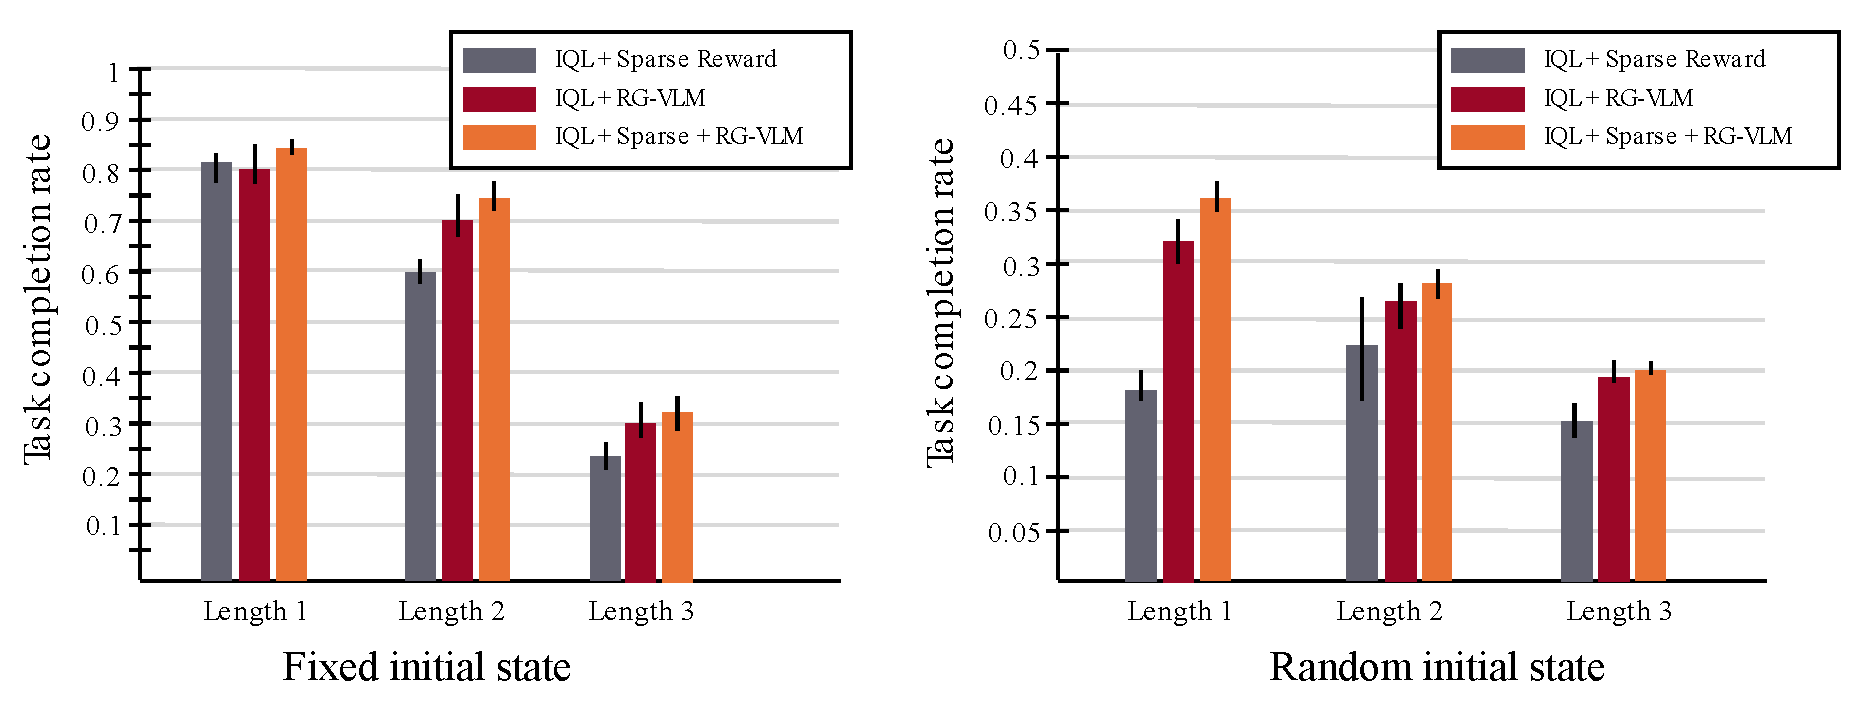
\includegraphics[width=16cm]{figures/figure9.pdf}
    \caption{Ablation study of reward design on ALFRED. We compare IQL trained with only the sparse environment reward, only the RG-VLM reward, and a combination of sparse + RG-VLM rewards under both fixed initial state (left) and random initial state (right) evaluation for instruction lengths 1–3. Across both settings, replacing the sparse reward with RG-VLM improves task completion rate, and combining RG-VLM with the sparse success signal yields the best performance,}
    \label{fig:exp_ablation}
\end{figure*}

\paragraph{Effect of RG-VLM as an Auxiliary Reward}
To investigate the potential of RG-VLM as an auxiliary reward signal, we compare three reward configurations on the ALFRED evaluation set: (i) training IQL with only the environment’s sparse success reward, (ii) training with only dense rewards generated by RG-VLM, and (iii) training with a combination of sparse and RG-VLM rewards. We evaluate tasks with one, two, and three subtasks. As shown in figure \ref{fig:exp_ablation}, the combined sparse and RG-VLM reward setting consistently achieves the highest task completion rates, outperforming both the sparse-only and RG-VLM-only configurations. This demonstrates that RG-VLM is also effective when used as an auxiliary shaping reward.

% \paragraph{Choice of LVLM}
% \begin{table}[h!]
% \centering
% \begin{tabular}{lcc}
% \toprule
% Model               & Accuracy (\%) & Inference Time (s) \\
% \midrule
% Gemini 1.5 Pro      & 93.4          & 26.6               \\
% Gemini 1.5 Flash    & 74.2          & 17.0               \\
% Qwen2-VL-72B        & 86.2          & 132.8              \\
% \bottomrule
% \end{tabular}
% \caption{Task completion accuracy and Inference time on 500 random trajectories with different LVLMs. Gemini models are called via public API and Qwen2-VL-72B is run on a single A100 GPU.}
% \label{tab:accuracy_tradeoff}
% \end{table}

% We also investigate how the choice of LVLM affects the quality and efficiency of reward generation in RG-VLM. To this end, we compare three different LVLM backbones within the same reward-generation pipeline: Gemini 1.5 Pro\cite{reid2024gemini}, Gemini 1.5 Flash\cite{reid2024gemini}, and Qwen2-VL-72B. For each model, we fix the prompt, window size, and all offline RL hyperparameters, and we measure (1) task completion accuracy of the resulting policy on 500 randomly sampled evaluation trajectories and (2) average inference time required to generate rewards for those trajectories. The results are summarized in Table \ref{tab:accuracy_tradeoff}.

% Gemini 1.5 Pro\cite{reid2024gemini} attains the highest task completion accuracy of 93.4\% with a moderate inference time of 26.6 seconds over 500 trajectories. In contrast, Gemini 1.5 Flash is faster, requiring only 17.0 seconds, but its accuracy drops to 74.2\%, indicating that the reduced model capacity harms the reliability of the generated rewards. Qwen2-VL-72B reaches an accuracy of 86.2\%, which is closer to Gemini 1.5 Pro, but it incurs a substantially higher inference time of 132.8 seconds when run on a single A100 GPU, making it less practical for large-scale offline datasets.

% These results highlight an important trade-off between reward quality and computational cost when selecting an LVLM for RG-VLM. Gemini 1.5 Flash offers low latency but generates noisier rewards that translate into weaker downstream RL performance. Qwen2-VL-72B provides reasonably strong rewards but is prohibitively slow for extensive offline datasets that contain tens of thousands of trajectories. Gemini 1.5 Pro, on the other hand, achieves the best balance between accuracy and inference time, delivering high-quality, semantically consistent rewards at a computational cost that remains feasible for large-scale experiments. For this reason, we adopt Gemini 1.5 Pro as the default LVLM backbone in all main RG-VLM experiments.

\paragraph{Effect of Prompt Design}
\begin{table}[h]
    \centering
    \setlength{\tabcolsep}{22pt}   % 열 사이 간격 (기본값보다 크게)
    \renewcommand{\arraystretch}{1.0} % 행 높이 늘리기

    % l : 왼쪽 정렬, X : 가변폭 열 (가운데 정렬)
    \begin{tabularx}{0.7\textwidth}{@{}rcc@{}}
        \toprule
        Prompt Setting                      & Accuracy & Recall \\
        \midrule
        No caption / No action       & 0.43     & 0.31   \\
        Use caption / No action      & 0.63     & 0.56   \\
        No caption / Use action      & 0.75     & 0.69   \\
        \textbf{Use caption / Use action} & \textbf{0.86} & \textbf{0.82} \\
        \bottomrule
    \end{tabularx}
    \caption{Task-success prediction accuracy and recall under different availability of caption and action information in the first query. “Caption” denotes the timestep text describing each observation image, and “Action” denotes the natural-language description of the executed action sequence.}
    \label{tab:prompt_ablation}
\end{table}

To validate our prompting design, we additionally analyze how different prompt components affect the LVLM’s ability to recognize successful trajectories. Using 100 random trajectories from ALFRED, we treat a trajectory as successful if the LVLM assigns a reward of 10 and compare the prediction against the environment’s sparse success label. As shown in table \ref{tab:prompt_ablation}, when neither per-frame caption (timestep text) nor action information is provided, the LVLM attains only 0.43 accuracy and 0.31 recall. Adding captions alone improves accuracy to 0.63 and recall to 0.56, while providing only the action sequence yields 0.75 accuracy and 0.69 recall. The full prompt, which includes both caption and action information, achieves 0.86 accuracy and 0.82 recall. This indicates that image sequences alone are insufficient to reliably determine whether a trajectory succeeds, whereas providing both captions and actions allows the model to capture task progress much more accurately. We observed that, without captions, the LVLM tends to skip certain timesteps when making its judgment, and without action information, the rewards for some actions are omitted. These findings confirm that the proposed prompt design substantially improves the quality of the rewards generated by the LVLM.

\paragraph{Correlation with Ground-truth Rewards} 
\begin{figure*}[h] 
    \centering 
    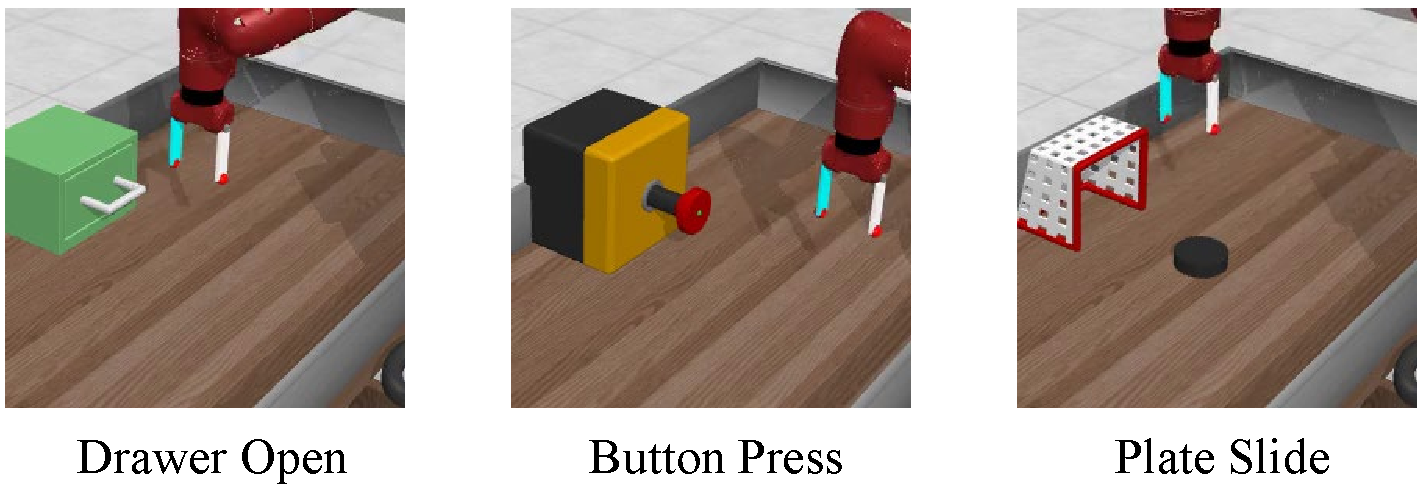
\includegraphics[width=10cm]{figures/figure10.pdf}
    \caption{Meta-World experimental environment. The Meta-World environment provides a real-valued reward between 0 and 1 at every step according to task progress.} 
    \label{fig:meta_ablation}
\end{figure*} 

\begin{figure*}[h] 
    \centering 
    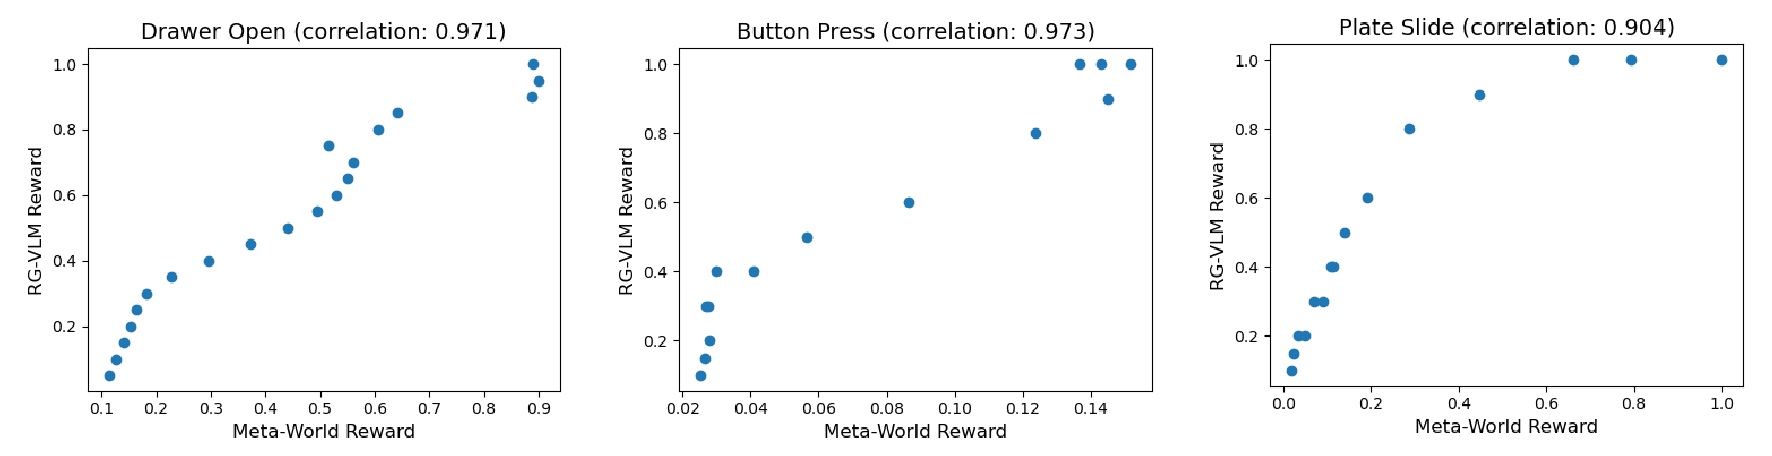
\includegraphics[width=16cm]{figures/figure11.pdf} 
    \caption{Scatter plots between the Meta-World ground-truth reward and the RG-VLM reward. As the ground-truth reward increases, the RG-VLM reward also increases, showing a positive correlation.} 
    \label{fig:meta_result_ablation} 
    \end{figure*} 

We conducted an experiment on three Meta-World tasks (Drawer Open, Button Press, and Plate Slide) as shown in Figure \ref{fig:meta_ablation} to compare the correlation between Meta-World’s ground-truth reward and the reward generated by RG-VLM. As shown in Figure \ref{fig:meta_result_ablation}, the resulting Pearson correlation coefficients are 0.971 for Drawer Open, 0.973 for Button Press, and 0.904 for Plate Slide, indicating a very strong positive correlation in all three tasks. This means that as the true environment reward increases, the RG-VLM reward also consistently increases, implying that the proposed reward aligns well with each trajectory’s task progress and that RG-VLM can generate meaningful reward signals even in real-world-like simulated environments such as Meta-World.


\chapter{Discussion}
In this thesis, we addressed the problem of reward specification in goal-conditioned offline reinforcement learning, where agents must learn from fixed datasets without any additional interaction with the environment. Designing dense, informative rewards for such datasets is notoriously labor-intensive and often requires substantial domain expertise, while standard sparse rewards provide little guidance for long-horizon tasks. To overcome this challenge, we proposed RG-VLM, a method that leverages Large Vision–Language Models (LVLMs) to automatically generate dense reward signals from offline trajectories and language instructions, without human-in-the-loop labeling.

RG-VLM operates in a two-stage prompting pipeline. In the first stage, the LVLM analyzes a window of visual observations and corresponding actions to infer the semantic structure of state transitions with respect to the language goal. In the second stage, conditioned on this contextualized analysis, the LVLM assigns step-wise reward scores that reflect each action’s contribution toward task completion. By sliding this window over the entire trajectory, RG-VLM produces a dense, interpretable reward sequence that can be directly used for offline RL training. We instantiate RG-VLM with Implicit Q-Learning (IQL), but the framework is compatible with any value-based offline RL algorithm.

Extensive experiments on the ALFRED benchmark demonstrate the effectiveness of our approach. Using a large-scale, diverse offline dataset consisting of 73k trajectories, 120 scenes, and 100 evaluation tasks spanning 65 scenes, we showed that RG-VLM significantly improves policy performance over strong baselines. When combined with sparse success rewards, IQL with RG-VLM consistently outperforms IQL with sparse rewards alone, as well as state-of-the-art VLM-based reward models such as CLIP-based VLM-RMs, BLIP2-based rewards, and RoboCLIP, across both fixed and randomized initial state settings and across task lengths from one to six subtasks. These results highlight that LVLM-generated dense rewards provide more informative learning signals, especially in long-horizon and distribution-shifted scenarios. 
%Ablation studies further confirm that using RG-VLM as an auxiliary shaping signal..
Ablation studies further confirm that (1) using RG-VLM as an auxiliary shaping signal, (2) the effectiveness of our prompt design, and (3) the strong correlation between RG-VLM rewards and ground-truth rewards.

The main contributions of this work are threefold. First, we introduce RG-VLM, a general framework for automated reward generation in offline RL that removes the need for manual reward engineering and human preference labeling. Second, we design a two-turn LVLM prompting strategy that explicitly separates transition understanding from reward assignment, enabling more accurate and interpretable dense reward generation. Third, through comprehensive experiments and ablations on ALFRED, we provide empirical evidence that LVLM-based dense rewards can substantially enhance policy learning and function effectively as auxiliary rewards on top of sparse task signals.

Despite these promising results, our study has several limitations that open up directions for future work. A first limitation is dataset coverage: we evaluate RG-VLM only on the ALFRED benchmark. Although ALFRED is large-scale and diverse, the generality of our findings remains to be confirmed on other language-annotated environments, such as BabyAI and CALVIN, and in domains beyond household manipulation. Extending RG-VLM to a broader range of tasks, including continuous-control and real-robot settings, is an important next step.

A second limitation concerns computational cost. LVLMs like Gemini 1.5 Pro, while providing high-quality rewards, incur non-trivial inference time during reward generation. In this work, we mitigate the cost by using a fixed window size and querying the LVLM offline, but the latency still poses challenges when scaling to even larger datasets or when repeated re-labeling is required. An appealing future direction is to use the LVLM only as a teacher to supervise a smaller, task-specific reward model or value estimator. Once trained, this distilled reward model could be used for fast reward evaluation during offline and online RL, thereby retaining the semantic richness of LVLM judgments while avoiding their runtime overhead. More broadly, integrating LVLM-derived supervision with learned reward models and theoretical analyses of their bias and generalization properties are promising avenues for future research.

In summary, this thesis demonstrates that LVLMs can serve as powerful reward designers for offline reinforcement learning. By converting high-level language goals and visual observations into dense, semantically grounded reward signals, RG-VLM bridges the gap between human task descriptions and low-level policy optimization. We hope that this work contributes a practical step toward scalable, human-aligned reward specification and inspires further exploration of LVLM-guided learning in both offline and online RL settings.



%%
%% 참고문헌 시작
%% bibliography
%% It can be changed but should include sufficient information.

\bibliographystyle{ieeetr}  % 원하는 스타일 유지
\bibliography{references}   % references.bib를 참조


%%
%% 감사의 글 시작
%% Acknowledgement
%%
% @command acknowledgement 감사의글
% @options [1 | 2 | 3 |4 ]
% - 1 : 본문과 감사의 글이 둘 다 한글일 때  | 2 : 본문은 한글인데 감사의 글이 영어일 때 | 3 :  본문과 감사의 글이 둘 다 영어일 때  | 4 : 본문은 영어인데 감사의 글이 % 한글일 때 
%% It is optional.

\acknowledgment[3]
ack


%%
%% 약력 시작
%% Curriculum Vitae
%%
% @command curriculumvitae 이력서
% @options [1 | 2 | 3 |4 ]
% - 1 : 본문과 약력이 둘 다 한글일 때  | 2 : 본문은 한글인데 약력이 영어일 때 | 3 :  본문과 약력이 둘 다 영어일 때  | 4 : 본문은 영어인데 약력이 한글일 때 
%% It is optional and you can change form of this in the class file if you want.
\curriculumvitae[3]

    % @environment personaldata 개인정보
    % @command     name         이름
    %              dateofbirth  생년월일
    %              birthplace   출생지
    %              domicile     본적지
    %              address      주소지
    %              email        E-mail 주소
    % - 위 6개의 기본 필드 중에 이력서에 적고 싶은 정보를 입력
    % input data only you want
    \begin{personaldata}
        \name       {Zheng Xuran}
        \dateofbirth{2002}{06}{13}
        % \address    {}
    \end{personaldata}

    % @environment education 학력
    % @options [default: (none)] - 수학기간을 입력
    \begin{education}
        % \item[2014. 3.\ --\ 2017. 2.] 
        \item[2020. 8.\ --\ 2024. 6.] Harbin Institute of Tecnology, Department of Computing (B.S.)
        \item[2024. 8.\ --\ 2027. 2.] Korea Advanced Institute of Science and Technology (KAIST), Department of Electrical Engineering (M.S.)
    \end{education}

    % @environment career 경력
    % @options [default: (none)] - 해당기간을 입력

    % @environment activity 학회활동
    % @options [default: (none)] - 활동내용을 입력
%%    \begin{activity}
%%        \item J. Choi, \textbf{Yong-Hyun Kim}, K.J. Chang, and D. Tomanek,
%%             \textit{Occurrence of itinerant ferromagnetism in C/BN superlattice
%%             nanotubes}, 5th Asian Workshop on First-Principles Electronic
%%             Structure Calculations, Seoul (Korea), October., 2002.
%%    \end{activity}

    % @environment publication 연구업적
    % @options [default: (none)] - 출판내용을 입력
    \begin{publication}
        %\item \textbf{Yong-Hyun Kim}, J. Choi, K.J. Chang, and D. Tomanek,
        %     \textit{Magnetic instability in partly opened C$_{60}$ isomers},
        %     in preparation.

% \item \textbf{Younghwan Lee*}, Tung Luu*, Donghoon Lee and Chang D. Yoo, "Reward Generation via Large Vision-Language Model in Offline Reinforcement Learning", The International Conference on Acoustics, Speech, \& Signal Processing (ICASSP) 2025.

% \item Sunjae Yoon, Gwanhyeong Koo, \textbf{Younghwan Lee} and Chang D. Yoo, "TPC: Test-time Procrustes Calibration for Diffusion-based Human Image Animation",  Neural Information Processing Systems (NeurIPS), 2024.

% \item Donghoon Lee*, Tung Luu*, \textbf{Younghwan Lee} and Chang D. Yoo, "Sample Efficient Reinforcement Learning via Large Vision Language Model Distillation", The International Conference on Acoustics, Speech, \& Signal Processing (ICASSP) 2025.

% \item Tung Minh Luu, \textbf{Younghwan Lee}, Donghoon Lee, Sunho Kim, Min Jun Kim and Chang D. Yoo, "Enhancing Rating-Based Reinforcement Learning to Effectively Leverage Feedback from Large Vision-Language Models", International Conference on Machine Learning (ICML), 2025

% \item Gwanhyeong Koo, Sunjae Yoon, \textbf{Younghwan Lee}, Ji Woo Hong and Chang D. Yoo, " FlowDrag: 3D-aware Drag-based Image Editing with Mesh-guided Deformation Vector Flow Fields", International Conference on Machine Learning (ICML), 2025.

% \item G. Tung Luu, Donghoon Lee, \textbf{Younghwan Lee} and Chang D. Yoo, "Policy Learning from Large Vision-Language Model Feedback Without Reward Modeling", The 2025 IEEE/RSJ International Conference on Intelligent Robots and Systems (IROS), 2025.

% \item Sunjae Yoon, Gwanhyeong Koo, \textbf{Younghwan Lee}, Ji Woo Hong and Chang D. Yoo, "Occlusion-robust Stylization for Drawing-based 3D Animation", International Conference on Computer Vision (ICCV) 2025.

    \end{publication}

  \label{paperlastpagelabel}     % <-- 추가 부분: 마지막 페이지 위치 지정	
%% 본문 끝
\end{document}
